\documentclass[twoside]{book}

% Packages required by doxygen
\usepackage{calc}
\usepackage{doxygen}
\usepackage{graphicx}
\usepackage[utf8]{inputenc}
\usepackage{makeidx}
\usepackage{multicol}
\usepackage{multirow}
\usepackage{textcomp}
\usepackage[table]{xcolor}

% Font selection
\usepackage[T1]{fontenc}
\usepackage{mathptmx}
\usepackage[scaled=.90]{helvet}
\usepackage{courier}
\usepackage{amssymb}
\usepackage{sectsty}
\renewcommand{\familydefault}{\sfdefault}
\allsectionsfont{%
  \fontseries{bc}\selectfont%
  \color{darkgray}%
}
\renewcommand{\DoxyLabelFont}{%
  \fontseries{bc}\selectfont%
  \color{darkgray}%
}

% Page & text layout
\usepackage{geometry}
\geometry{%
  a4paper,%
  top=2.5cm,%
  bottom=2.5cm,%
  left=2.5cm,%
  right=2.5cm%
}
\tolerance=750
\hfuzz=15pt
\hbadness=750
\setlength{\emergencystretch}{15pt}
\setlength{\parindent}{0cm}
\setlength{\parskip}{0.2cm}
\makeatletter
\renewcommand{\paragraph}{%
  \@startsection{paragraph}{4}{0ex}{-1.0ex}{1.0ex}{%
    \normalfont\normalsize\bfseries\SS@parafont%
  }%
}
\renewcommand{\subparagraph}{%
  \@startsection{subparagraph}{5}{0ex}{-1.0ex}{1.0ex}{%
    \normalfont\normalsize\bfseries\SS@subparafont%
  }%
}
\makeatother

% Headers & footers
\usepackage{fancyhdr}
\pagestyle{fancyplain}
\fancyhead[LE]{\fancyplain{}{\bfseries\thepage}}
\fancyhead[CE]{\fancyplain{}{}}
\fancyhead[RE]{\fancyplain{}{\bfseries\leftmark}}
\fancyhead[LO]{\fancyplain{}{\bfseries\rightmark}}
\fancyhead[CO]{\fancyplain{}{}}
\fancyhead[RO]{\fancyplain{}{\bfseries\thepage}}
\fancyfoot[LE]{\fancyplain{}{}}
\fancyfoot[CE]{\fancyplain{}{}}
\fancyfoot[RE]{\fancyplain{}{\bfseries\scriptsize Generated on Thu Apr 2 2015 17\-:59\-:42 for Lightweight Dynamic Memory Manager by Doxygen }}
\fancyfoot[LO]{\fancyplain{}{\bfseries\scriptsize Generated on Thu Apr 2 2015 17\-:59\-:42 for Lightweight Dynamic Memory Manager by Doxygen }}
\fancyfoot[CO]{\fancyplain{}{}}
\fancyfoot[RO]{\fancyplain{}{}}
\renewcommand{\footrulewidth}{0.4pt}
\renewcommand{\chaptermark}[1]{%
  \markboth{#1}{}%
}
\renewcommand{\sectionmark}[1]{%
  \markright{\thesection\ #1}%
}

% Indices & bibliography
\usepackage{natbib}
\usepackage[titles]{tocloft}
\setcounter{tocdepth}{3}
\setcounter{secnumdepth}{5}
\makeindex

% Hyperlinks (required, but should be loaded last)
\usepackage{ifpdf}
\ifpdf
  \usepackage[pdftex,pagebackref=true]{hyperref}
\else
  \usepackage[ps2pdf,pagebackref=true]{hyperref}
\fi
\hypersetup{%
  colorlinks=true,%
  linkcolor=blue,%
  citecolor=blue,%
  unicode%
}

% Custom commands
\newcommand{\clearemptydoublepage}{%
  \newpage{\pagestyle{empty}\cleardoublepage}%
}


%===== C O N T E N T S =====

\begin{document}

% Titlepage & ToC
\hypersetup{pageanchor=false}
\pagenumbering{roman}
\begin{titlepage}
\vspace*{7cm}
\begin{center}%
{\Large Lightweight Dynamic Memory Manager \\[1ex]\large stable-\/version-\/v-\/1.\-3 }\\
\vspace*{1cm}
{\large Generated by Doxygen 1.8.6}\\
\vspace*{0.5cm}
{\small Thu Apr 2 2015 17:59:42}\\
\end{center}
\end{titlepage}
\clearemptydoublepage
\tableofcontents
\clearemptydoublepage
\pagenumbering{arabic}
\hypersetup{pageanchor=true}

%--- Begin generated contents ---
\chapter{Hierarchical Index}
\section{Class Hierarchy}
This inheritance list is sorted roughly, but not completely, alphabetically\-:\begin{DoxyCompactList}
\item Crazy\-Thread\begin{DoxyCompactList}
\item \contentsline{section}{Garbage\-Collector\-Thread}{\pageref{class_garbage_collector_thread}}{}
\item \contentsline{section}{memory\-Compactor}{\pageref{classmemory_compactor}}{}
\end{DoxyCompactList}
\item \contentsline{section}{Exploration\-V\-Heap}{\pageref{class_exploration_v_heap}}{}
\item \contentsline{section}{Minimalism\-Bit\-Vector}{\pageref{class_minimalism_bit_vector}}{}
\item \contentsline{section}{v\-Char}{\pageref{classv_char}}{}
\item \contentsline{section}{v\-Heap}{\pageref{classv_heap}}{}
\item \contentsline{section}{V\-Heap\-Exception}{\pageref{class_v_heap_exception}}{}
\begin{DoxyCompactList}
\item \contentsline{section}{Full\-Memory\-Heap\-Exception}{\pageref{class_full_memory_heap_exception}}{}
\item \contentsline{section}{No\-Match\-Classes\-Exception}{\pageref{class_no_match_classes_exception}}{}
\item \contentsline{section}{Null\-Pointer\-Exception}{\pageref{class_null_pointer_exception}}{}
\end{DoxyCompactList}
\item \contentsline{section}{v\-Object}{\pageref{classv_object}}{}
\begin{DoxyCompactList}
\item \contentsline{section}{v\-Int}{\pageref{classv_int}}{}
\end{DoxyCompactList}
\item \contentsline{section}{v\-Ref}{\pageref{classv_ref}}{}
\end{DoxyCompactList}

\chapter{Class Index}
\section{Class List}
Here are the classes, structs, unions and interfaces with brief descriptions\-:\begin{DoxyCompactList}
\item\contentsline{section}{\hyperlink{class_exploration_v_heap}{Exploration\-V\-Heap} }{\pageref{class_exploration_v_heap}}{}
\item\contentsline{section}{\hyperlink{class_full_memory_heap_exception}{Full\-Memory\-Heap\-Exception} \\*Es la clase que representa el error de memoria llena }{\pageref{class_full_memory_heap_exception}}{}
\item\contentsline{section}{\hyperlink{class_garbage_collector_thread}{Garbage\-Collector\-Thread} \\*Es la clase que se encarga de borrar los elementos no referenciados }{\pageref{class_garbage_collector_thread}}{}
\item\contentsline{section}{\hyperlink{classmemory_compactor}{memory\-Compactor} \\*Es la clase que se encarga de realizar la compactacion de los datos en el \hyperlink{classv_heap}{v\-Heap} }{\pageref{classmemory_compactor}}{}
\item\contentsline{section}{\hyperlink{class_minimalism_bit_vector}{Minimalism\-Bit\-Vector} }{\pageref{class_minimalism_bit_vector}}{}
\item\contentsline{section}{\hyperlink{class_no_match_classes_exception}{No\-Match\-Classes\-Exception} \\*Es la clase que representa al error cuando dos objeto no pertenecen a la misma clase }{\pageref{class_no_match_classes_exception}}{}
\item\contentsline{section}{\hyperlink{class_null_pointer_exception}{Null\-Pointer\-Exception} \\*La clase \hyperlink{class_null_pointer_exception}{Null\-Pointer\-Exception}, representa al error que se envia cuando se accesa a una porcion de memoria a la cual no se puede accesar }{\pageref{class_null_pointer_exception}}{}
\item\contentsline{section}{\hyperlink{classv_char}{v\-Char} }{\pageref{classv_char}}{}
\item\contentsline{section}{\hyperlink{classv_heap}{v\-Heap} \\*La clase \hyperlink{classv_heap}{v\-Heap}, Representa a un manejador de memoria. Cuenta con un compresor de memoria, garbage collector y los metodos escenciales }{\pageref{classv_heap}}{}
\item\contentsline{section}{\hyperlink{class_v_heap_exception}{V\-Heap\-Exception} \\*La clase \hyperlink{class_v_heap_exception}{V\-Heap\-Exception}, Representa cualquier error generado por el \hyperlink{classv_heap}{v\-Heap} }{\pageref{class_v_heap_exception}}{}
\item\contentsline{section}{\hyperlink{classv_int}{v\-Int} \\*Es la clase que representa al int comun }{\pageref{classv_int}}{}
\item\contentsline{section}{\hyperlink{classv_object}{v\-Object} \\*Es la clase que representa al objeto contenido en el \hyperlink{classv_heap}{v\-Heap} }{\pageref{classv_object}}{}
\item\contentsline{section}{\hyperlink{classv_ref}{v\-Ref} }{\pageref{classv_ref}}{}
\end{DoxyCompactList}

\chapter{Class Documentation}
\hypertarget{class_exploration_v_heap}{\section{Exploration\-V\-Heap Class Reference}
\label{class_exploration_v_heap}\index{Exploration\-V\-Heap@{Exploration\-V\-Heap}}
}


The documentation for this class was generated from the following file\-:\begin{DoxyCompactItemize}
\item 
src/vheap.\-cpp\end{DoxyCompactItemize}

\hypertarget{class_full_memory_heap_exception}{\section{Full\-Memory\-Heap\-Exception Class Reference}
\label{class_full_memory_heap_exception}\index{Full\-Memory\-Heap\-Exception@{Full\-Memory\-Heap\-Exception}}
}


Es la clase que representa el error de memoria llena.  




{\ttfamily \#include $<$fullmemoryexception.\-h$>$}

Inheritance diagram for Full\-Memory\-Heap\-Exception\-:\begin{figure}[H]
\begin{center}
\leavevmode
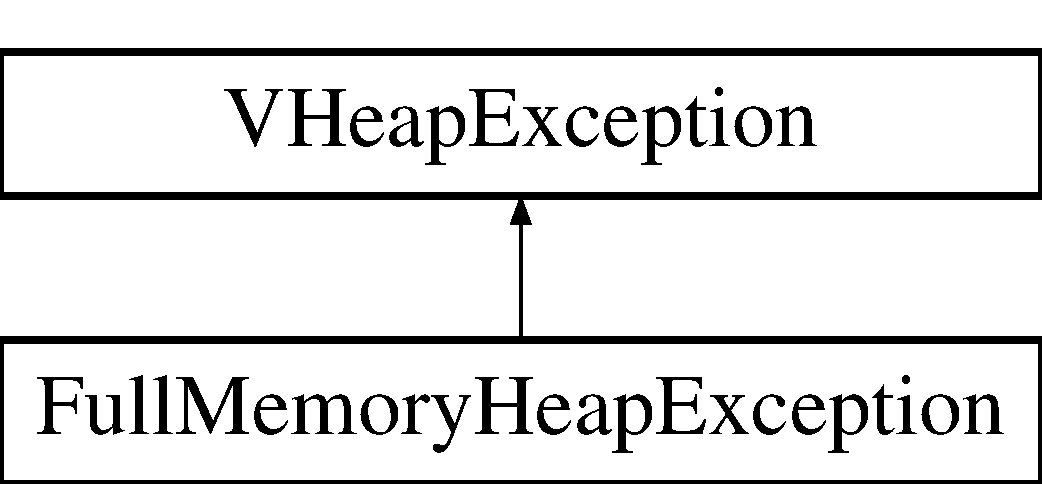
\includegraphics[height=2.000000cm]{class_full_memory_heap_exception}
\end{center}
\end{figure}
\subsection*{Public Member Functions}
\begin{DoxyCompactItemize}
\item 
const char $\ast$ \hyperlink{class_full_memory_heap_exception_a66ee760289cae528c31ffdedfc2ccc0a}{what} ()
\begin{DoxyCompactList}\small\item\em Es el metodo que contiene el mensaje de error de la clase. \end{DoxyCompactList}\end{DoxyCompactItemize}


\subsection{Detailed Description}
Es la clase que representa el error de memoria llena. 

\subsection{Member Function Documentation}
\hypertarget{class_full_memory_heap_exception_a66ee760289cae528c31ffdedfc2ccc0a}{\index{Full\-Memory\-Heap\-Exception@{Full\-Memory\-Heap\-Exception}!what@{what}}
\index{what@{what}!FullMemoryHeapException@{Full\-Memory\-Heap\-Exception}}
\subsubsection[{what}]{\setlength{\rightskip}{0pt plus 5cm}const char$\ast$ Full\-Memory\-Heap\-Exception\-::what (
\begin{DoxyParamCaption}
{}
\end{DoxyParamCaption}
)\hspace{0.3cm}{\ttfamily [inline]}, {\ttfamily [virtual]}}}\label{class_full_memory_heap_exception_a66ee760289cae528c31ffdedfc2ccc0a}


Es el metodo que contiene el mensaje de error de la clase. 

\begin{DoxyReturn}{Returns}
una cadena de caracteres que contiene el error 
\end{DoxyReturn}


Reimplemented from \hyperlink{class_v_heap_exception_a58154e8dc02f9c28dfefad7897f8b2cf}{V\-Heap\-Exception}.



The documentation for this class was generated from the following file\-:\begin{DoxyCompactItemize}
\item 
src/fullmemoryexception.\-h\end{DoxyCompactItemize}

\hypertarget{class_garbage_collector_thread}{\section{Garbage\-Collector\-Thread Class Reference}
\label{class_garbage_collector_thread}\index{Garbage\-Collector\-Thread@{Garbage\-Collector\-Thread}}
}


Es la clase que se encarga de borrar los elementos no referenciados.  




{\ttfamily \#include $<$garbagecollectorthread.\-h$>$}

Inheritance diagram for Garbage\-Collector\-Thread\-:\begin{figure}[H]
\begin{center}
\leavevmode
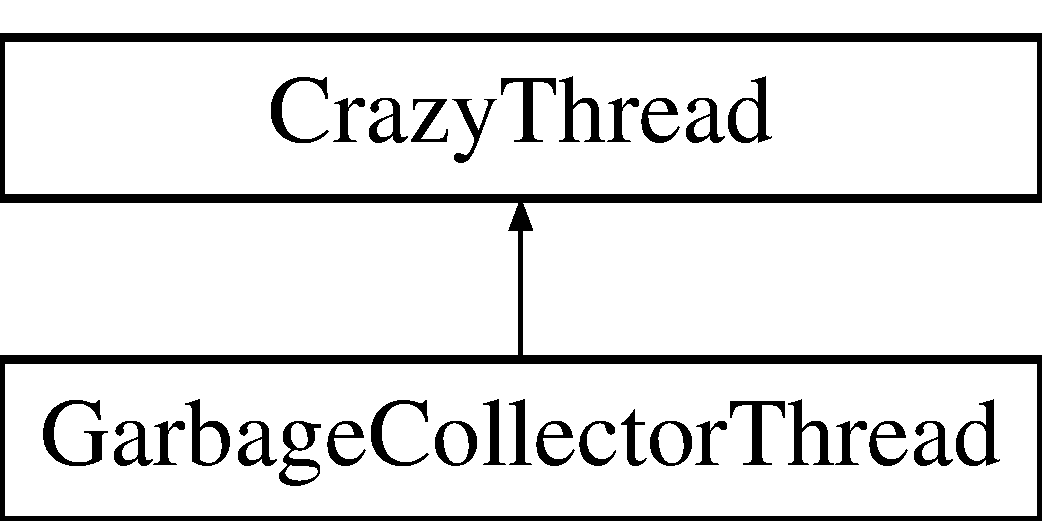
\includegraphics[height=2.000000cm]{class_garbage_collector_thread}
\end{center}
\end{figure}
\subsection*{Public Member Functions}
\begin{DoxyCompactItemize}
\item 
\hyperlink{class_garbage_collector_thread_a0c4840e9a065994f8fcd61098ddc5fe0}{Garbage\-Collector\-Thread} (unsigned int p\-Time\-To\-Wait)
\begin{DoxyCompactList}\small\item\em Incializa el valor de espera del thread. \end{DoxyCompactList}\end{DoxyCompactItemize}
\subsection*{Protected Member Functions}
\begin{DoxyCompactItemize}
\item 
\hypertarget{class_garbage_collector_thread_a83e5fd4ed87eff4383e60960cf34854b}{void {\bfseries internal\-Run} ()}\label{class_garbage_collector_thread_a83e5fd4ed87eff4383e60960cf34854b}

\end{DoxyCompactItemize}


\subsection{Detailed Description}
Es la clase que se encarga de borrar los elementos no referenciados. 

\subsection{Constructor \& Destructor Documentation}
\hypertarget{class_garbage_collector_thread_a0c4840e9a065994f8fcd61098ddc5fe0}{\index{Garbage\-Collector\-Thread@{Garbage\-Collector\-Thread}!Garbage\-Collector\-Thread@{Garbage\-Collector\-Thread}}
\index{Garbage\-Collector\-Thread@{Garbage\-Collector\-Thread}!GarbageCollectorThread@{Garbage\-Collector\-Thread}}
\subsubsection[{Garbage\-Collector\-Thread}]{\setlength{\rightskip}{0pt plus 5cm}Garbage\-Collector\-Thread\-::\-Garbage\-Collector\-Thread (
\begin{DoxyParamCaption}
\item[{unsigned int}]{p\-Time\-To\-Wait}
\end{DoxyParamCaption}
)}}\label{class_garbage_collector_thread_a0c4840e9a065994f8fcd61098ddc5fe0}


Incializa el valor de espera del thread. 


\begin{DoxyParams}{Parameters}
{\em p\-Time\-To\-Wait} & Es la cantidad de tiempo que espera el thread hasta despertarse de nuevo, la cantidad de tiempo es en milisegundos \\
\hline
\end{DoxyParams}


The documentation for this class was generated from the following files\-:\begin{DoxyCompactItemize}
\item 
src/garbagecollectorthread.\-h\item 
src/garbagecollectorthread.\-cpp\end{DoxyCompactItemize}

\hypertarget{classmemory_compactor}{\section{memory\-Compactor Class Reference}
\label{classmemory_compactor}\index{memory\-Compactor@{memory\-Compactor}}
}


Es la clase que se encarga de realizar la compactacion de los datos en el \hyperlink{classv_heap}{v\-Heap}.  




{\ttfamily \#include $<$memorycompactor.\-h$>$}

Inheritance diagram for memory\-Compactor\-:\begin{figure}[H]
\begin{center}
\leavevmode
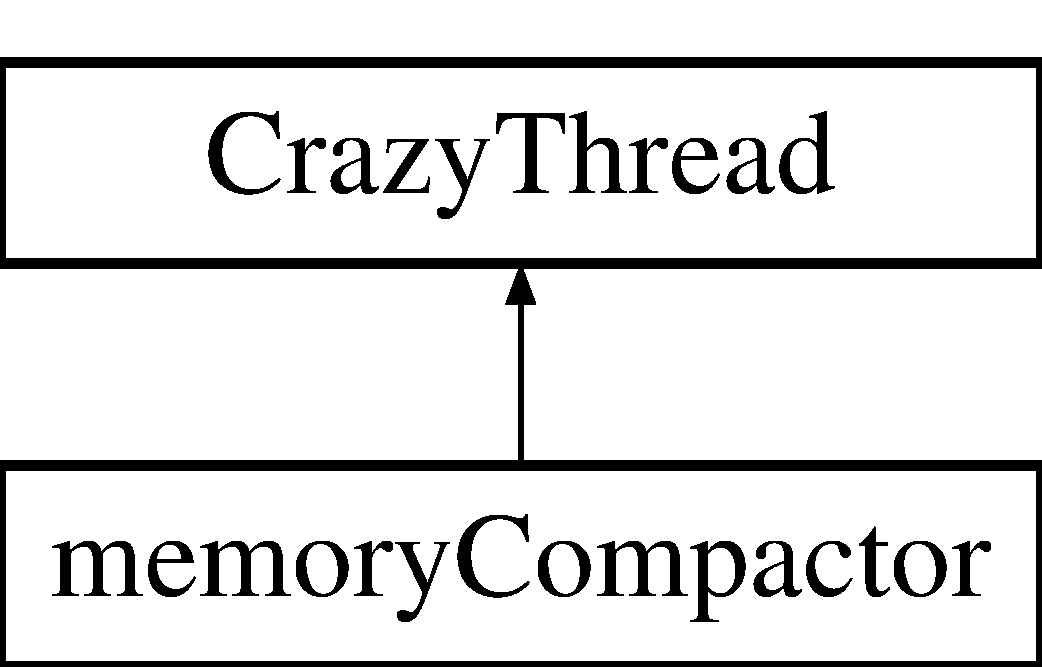
\includegraphics[height=2.000000cm]{classmemory_compactor}
\end{center}
\end{figure}
\subsection*{Public Member Functions}
\begin{DoxyCompactItemize}
\item 
\hyperlink{classmemory_compactor_a4aafa6e4c651ff8c50ca2fc14e32d7eb}{memory\-Compactor} (unsigned int p\-Time\-To\-Sleep)
\begin{DoxyCompactList}\small\item\em Inicializa el objeto, y ademas el tiempo que el thread va a dormir. \end{DoxyCompactList}\end{DoxyCompactItemize}
\subsection*{Protected Member Functions}
\begin{DoxyCompactItemize}
\item 
\hypertarget{classmemory_compactor_ac7ff9969c2f8d4abddb85317aaba757e}{void {\bfseries internal\-Run} ()}\label{classmemory_compactor_ac7ff9969c2f8d4abddb85317aaba757e}

\end{DoxyCompactItemize}


\subsection{Detailed Description}
Es la clase que se encarga de realizar la compactacion de los datos en el \hyperlink{classv_heap}{v\-Heap}. 

\subsection{Constructor \& Destructor Documentation}
\hypertarget{classmemory_compactor_a4aafa6e4c651ff8c50ca2fc14e32d7eb}{\index{memory\-Compactor@{memory\-Compactor}!memory\-Compactor@{memory\-Compactor}}
\index{memory\-Compactor@{memory\-Compactor}!memoryCompactor@{memory\-Compactor}}
\subsubsection[{memory\-Compactor}]{\setlength{\rightskip}{0pt plus 5cm}memory\-Compactor\-::memory\-Compactor (
\begin{DoxyParamCaption}
\item[{unsigned int}]{p\-Time\-To\-Sleep}
\end{DoxyParamCaption}
)}}\label{classmemory_compactor_a4aafa6e4c651ff8c50ca2fc14e32d7eb}


Inicializa el objeto, y ademas el tiempo que el thread va a dormir. 


\begin{DoxyParams}{Parameters}
{\em p\-Time\-To\-Sleep} & es la cantidad de tiempo que dura el thread en dormir el tiempo es en milisegundos \\
\hline
\end{DoxyParams}


The documentation for this class was generated from the following files\-:\begin{DoxyCompactItemize}
\item 
src/memorycompactor.\-h\item 
src/memorycompactor.\-cpp\end{DoxyCompactItemize}

\hypertarget{class_minimalism_bit_vector}{\section{Minimalism\-Bit\-Vector Class Reference}
\label{class_minimalism_bit_vector}\index{Minimalism\-Bit\-Vector@{Minimalism\-Bit\-Vector}}
}
\subsection*{Public Member Functions}
\begin{DoxyCompactItemize}
\item 
\hypertarget{class_minimalism_bit_vector_a86a42058658485f11691aa7d73f89197}{{\bfseries Minimalism\-Bit\-Vector} (const \hyperlink{class_minimalism_bit_vector}{Minimalism\-Bit\-Vector} \&othervariable)}\label{class_minimalism_bit_vector_a86a42058658485f11691aa7d73f89197}

\item 
\hyperlink{class_minimalism_bit_vector_a34fbf98499cea153210a7281fd093d88}{Minimalism\-Bit\-Vector} (unsigned int p\-Offset, unsigned int p\-Weight)
\begin{DoxyCompactList}\small\item\em Constructor de los objetos de la clase, inicializa las variables principales tales variables son aquellas que describen las principales caracteristicas de los objetos en memoria, tales caracteristicas son\-: el offset o direccion relativa, esta se mide en bytes y el corriemiento de bytes se da de 1 en 1, el peso del objeto y finalmente el tipo del objeto. \end{DoxyCompactList}\item 
\hypertarget{class_minimalism_bit_vector_a77e8a538b975ae40aa2205e4bedb6d09}{void \hyperlink{class_minimalism_bit_vector_a77e8a538b975ae40aa2205e4bedb6d09}{add\-Reference} ()}\label{class_minimalism_bit_vector_a77e8a538b975ae40aa2205e4bedb6d09}

\begin{DoxyCompactList}\small\item\em suma en uno al contador de referencia \end{DoxyCompactList}\item 
\hypertarget{class_minimalism_bit_vector_ace33d25bceb2a3c4c2e2820650c37e10}{void \hyperlink{class_minimalism_bit_vector_ace33d25bceb2a3c4c2e2820650c37e10}{remove\-Reference} ()}\label{class_minimalism_bit_vector_ace33d25bceb2a3c4c2e2820650c37e10}

\begin{DoxyCompactList}\small\item\em resta en uno el contador de referencias \end{DoxyCompactList}\item 
bool \hyperlink{class_minimalism_bit_vector_aa8bba4e5bcfae52caf3c99beb7aae0cf}{is\-Charged\-On\-Memory} () const 
\begin{DoxyCompactList}\small\item\em Verifica si el objeto que se representa a travez de las instancias de \hyperlink{class_minimalism_bit_vector}{Minimalism\-Bit\-Vector} estan cargadas en memoria. \end{DoxyCompactList}\item 
bool \hyperlink{class_minimalism_bit_vector_a7ebf4e232220001d18be6275d9868587}{is\-On\-Use} () const 
\begin{DoxyCompactList}\small\item\em Verifica si el objeto esta siendo usado por algun otro recurso. \end{DoxyCompactList}\item 
void \hyperlink{class_minimalism_bit_vector_a63b95b7f8446bfc105d42837be83b42b}{set\-On\-Use} (bool p\-On\-Use)
\begin{DoxyCompactList}\small\item\em setea la bandera que indica si el objeto se esta usando, true si se quiere que el objeto este en uso, false si se quiere que el objeto ya no este en uso. \end{DoxyCompactList}\item 
void \hyperlink{class_minimalism_bit_vector_a747ed61c44f091dd3326644216a923dd}{set\-On\-Memory\-Location} (bool p\-Memory\-Location\-Flag)
\begin{DoxyCompactList}\small\item\em Setea si el dato esta en memoria, si se quiere que el dato este en memoria se pasa el valor true por parametro en caso contrario se pasa un false. \end{DoxyCompactList}\item 
unsigned int \hyperlink{class_minimalism_bit_vector_af33224c672b353285b59463c2e958061}{get\-Weight} () const 
\begin{DoxyCompactList}\small\item\em obtiene el peso del objeto que representa \end{DoxyCompactList}\item 
void \hyperlink{class_minimalism_bit_vector_ac4480ef294435f54049da5cad957e1a9}{set\-Weight} (unsigned int p\-Weight)
\begin{DoxyCompactList}\small\item\em setea el peso del objeto al cual repesenta \end{DoxyCompactList}\item 
int \hyperlink{class_minimalism_bit_vector_a166c2b2c6e84945e329310584ca89128}{get\-Id} () const 
\begin{DoxyCompactList}\small\item\em obtiene el el id del objeto \end{DoxyCompactList}\item 
unsigned int \hyperlink{class_minimalism_bit_vector_ae17a440748037ed78b67bf9a2f4aad1d}{get\-Offset} () const 
\begin{DoxyCompactList}\small\item\em retorna el movimiento relativo en memoria desde el inicio del \hyperlink{classv_heap}{v\-Heap} \end{DoxyCompactList}\item 
void \hyperlink{class_minimalism_bit_vector_ad9d6993d2a24b1f238f1896dd8ff04be}{set\-Offset} (unsigned int p\-Offset)
\begin{DoxyCompactList}\small\item\em setea el offset al cual representa este objeto \end{DoxyCompactList}\item 
int \hyperlink{class_minimalism_bit_vector_ab0c91d2ff39599b96ba7f0c52ed796d2}{get\-Reference\-Counter} () const 
\begin{DoxyCompactList}\small\item\em Obtiene la cantidad de referencias al cual este objeto, representa. \end{DoxyCompactList}\item 
void \hyperlink{class_minimalism_bit_vector_af65272b7663cfc96d2a8fd16668b8570}{set\-Reference\-Counter} (int p\-Reference\-Counter)
\begin{DoxyCompactList}\small\item\em Setea la cantidad de referencias al objeto. \end{DoxyCompactList}\item 
bool \hyperlink{class_minimalism_bit_vector_ab6073c581675be3a1a8837aea19babb0}{operator$<$} (const \hyperlink{class_minimalism_bit_vector}{Minimalism\-Bit\-Vector} \&other\-Bit\-Vector)
\begin{DoxyCompactList}\small\item\em operator $<$, se compara con otro objeto a partir de su offset \end{DoxyCompactList}\item 
bool \hyperlink{class_minimalism_bit_vector_ae81b007ae02dc1263bda1bc0d217c125}{operator$>$} (const \hyperlink{class_minimalism_bit_vector}{Minimalism\-Bit\-Vector} \&other\-Bit\-Vector)
\begin{DoxyCompactList}\small\item\em operator $<$, se compara con otro objeto a partir de su offset \end{DoxyCompactList}\item 
bool \hyperlink{class_minimalism_bit_vector_afa354ed29c29fcea2bfc453aa2edb9e7}{operator!=} (const \hyperlink{class_minimalism_bit_vector}{Minimalism\-Bit\-Vector} \&other\-Bit\-Vector)
\begin{DoxyCompactList}\small\item\em operator $>$, se compara con otro objeto a partir de su offset \end{DoxyCompactList}\item 
\hypertarget{class_minimalism_bit_vector_a3c8458d181a7dedc5fe95d4e4cc1667a}{virtual \hyperlink{class_minimalism_bit_vector_a3c8458d181a7dedc5fe95d4e4cc1667a}{$\sim$\-Minimalism\-Bit\-Vector} ()}\label{class_minimalism_bit_vector_a3c8458d181a7dedc5fe95d4e4cc1667a}

\begin{DoxyCompactList}\small\item\em destructor o liberador de memoria \end{DoxyCompactList}\end{DoxyCompactItemize}
\subsection*{Friends}
\begin{DoxyCompactItemize}
\item 
ostream \& \hyperlink{class_minimalism_bit_vector_ab3123b16267666cc75c71b1cfb9a8a52}{operator$<$$<$} (ostream \&os, const \hyperlink{class_minimalism_bit_vector}{Minimalism\-Bit\-Vector} \&e)
\begin{DoxyCompactList}\small\item\em operator !=, se compara con otro objeto a partir de su offset \end{DoxyCompactList}\end{DoxyCompactItemize}


\subsection{Constructor \& Destructor Documentation}
\hypertarget{class_minimalism_bit_vector_a34fbf98499cea153210a7281fd093d88}{\index{Minimalism\-Bit\-Vector@{Minimalism\-Bit\-Vector}!Minimalism\-Bit\-Vector@{Minimalism\-Bit\-Vector}}
\index{Minimalism\-Bit\-Vector@{Minimalism\-Bit\-Vector}!MinimalismBitVector@{Minimalism\-Bit\-Vector}}
\subsubsection[{Minimalism\-Bit\-Vector}]{\setlength{\rightskip}{0pt plus 5cm}Minimalism\-Bit\-Vector\-::\-Minimalism\-Bit\-Vector (
\begin{DoxyParamCaption}
\item[{unsigned int}]{p\-Offset, }
\item[{unsigned int}]{p\-Weight}
\end{DoxyParamCaption}
)}}\label{class_minimalism_bit_vector_a34fbf98499cea153210a7281fd093d88}


Constructor de los objetos de la clase, inicializa las variables principales tales variables son aquellas que describen las principales caracteristicas de los objetos en memoria, tales caracteristicas son\-: el offset o direccion relativa, esta se mide en bytes y el corriemiento de bytes se da de 1 en 1, el peso del objeto y finalmente el tipo del objeto. 


\begin{DoxyParams}{Parameters}
{\em p\-Offset} & es la ubicacion del objeto que ademas es el identificador unico de cada una de las variables en memoria virtual, debido a que los objetos no pueden compartir la misma direccion de memoria. \\
\hline
{\em p\-Weight} & es el tamanio del objeto al cual representa el objeto instanciado \\
\hline
{\em p\-Type} & es el tipo del objeto al cual esta clase representa. \\
\hline
\end{DoxyParams}


\subsection{Member Function Documentation}
\hypertarget{class_minimalism_bit_vector_a166c2b2c6e84945e329310584ca89128}{\index{Minimalism\-Bit\-Vector@{Minimalism\-Bit\-Vector}!get\-Id@{get\-Id}}
\index{get\-Id@{get\-Id}!MinimalismBitVector@{Minimalism\-Bit\-Vector}}
\subsubsection[{get\-Id}]{\setlength{\rightskip}{0pt plus 5cm}int Minimalism\-Bit\-Vector\-::get\-Id (
\begin{DoxyParamCaption}
{}
\end{DoxyParamCaption}
) const}}\label{class_minimalism_bit_vector_a166c2b2c6e84945e329310584ca89128}


obtiene el el id del objeto 

\begin{DoxyReturn}{Returns}
el id del objeto 
\end{DoxyReturn}
\hypertarget{class_minimalism_bit_vector_ae17a440748037ed78b67bf9a2f4aad1d}{\index{Minimalism\-Bit\-Vector@{Minimalism\-Bit\-Vector}!get\-Offset@{get\-Offset}}
\index{get\-Offset@{get\-Offset}!MinimalismBitVector@{Minimalism\-Bit\-Vector}}
\subsubsection[{get\-Offset}]{\setlength{\rightskip}{0pt plus 5cm}unsigned int Minimalism\-Bit\-Vector\-::get\-Offset (
\begin{DoxyParamCaption}
{}
\end{DoxyParamCaption}
) const}}\label{class_minimalism_bit_vector_ae17a440748037ed78b67bf9a2f4aad1d}


retorna el movimiento relativo en memoria desde el inicio del \hyperlink{classv_heap}{v\-Heap} 

\begin{DoxyReturn}{Returns}
el \char`\"{}offset\char`\"{} del dato al cual este representa 
\end{DoxyReturn}
\hypertarget{class_minimalism_bit_vector_ab0c91d2ff39599b96ba7f0c52ed796d2}{\index{Minimalism\-Bit\-Vector@{Minimalism\-Bit\-Vector}!get\-Reference\-Counter@{get\-Reference\-Counter}}
\index{get\-Reference\-Counter@{get\-Reference\-Counter}!MinimalismBitVector@{Minimalism\-Bit\-Vector}}
\subsubsection[{get\-Reference\-Counter}]{\setlength{\rightskip}{0pt plus 5cm}int Minimalism\-Bit\-Vector\-::get\-Reference\-Counter (
\begin{DoxyParamCaption}
{}
\end{DoxyParamCaption}
) const}}\label{class_minimalism_bit_vector_ab0c91d2ff39599b96ba7f0c52ed796d2}


Obtiene la cantidad de referencias al cual este objeto, representa. 

\begin{DoxyReturn}{Returns}
la cantidad de referencias al objeto que representa 
\end{DoxyReturn}
\hypertarget{class_minimalism_bit_vector_af33224c672b353285b59463c2e958061}{\index{Minimalism\-Bit\-Vector@{Minimalism\-Bit\-Vector}!get\-Weight@{get\-Weight}}
\index{get\-Weight@{get\-Weight}!MinimalismBitVector@{Minimalism\-Bit\-Vector}}
\subsubsection[{get\-Weight}]{\setlength{\rightskip}{0pt plus 5cm}unsigned int Minimalism\-Bit\-Vector\-::get\-Weight (
\begin{DoxyParamCaption}
{}
\end{DoxyParamCaption}
) const}}\label{class_minimalism_bit_vector_af33224c672b353285b59463c2e958061}


obtiene el peso del objeto que representa 

\begin{DoxyReturn}{Returns}
el peso del objeto al cual representa 
\end{DoxyReturn}
\hypertarget{class_minimalism_bit_vector_aa8bba4e5bcfae52caf3c99beb7aae0cf}{\index{Minimalism\-Bit\-Vector@{Minimalism\-Bit\-Vector}!is\-Charged\-On\-Memory@{is\-Charged\-On\-Memory}}
\index{is\-Charged\-On\-Memory@{is\-Charged\-On\-Memory}!MinimalismBitVector@{Minimalism\-Bit\-Vector}}
\subsubsection[{is\-Charged\-On\-Memory}]{\setlength{\rightskip}{0pt plus 5cm}bool Minimalism\-Bit\-Vector\-::is\-Charged\-On\-Memory (
\begin{DoxyParamCaption}
{}
\end{DoxyParamCaption}
) const}}\label{class_minimalism_bit_vector_aa8bba4e5bcfae52caf3c99beb7aae0cf}


Verifica si el objeto que se representa a travez de las instancias de \hyperlink{class_minimalism_bit_vector}{Minimalism\-Bit\-Vector} estan cargadas en memoria. 

\begin{DoxyReturn}{Returns}
true, si el objeto esta en memoria, false si el objeto esta en disco 
\end{DoxyReturn}
\hypertarget{class_minimalism_bit_vector_a7ebf4e232220001d18be6275d9868587}{\index{Minimalism\-Bit\-Vector@{Minimalism\-Bit\-Vector}!is\-On\-Use@{is\-On\-Use}}
\index{is\-On\-Use@{is\-On\-Use}!MinimalismBitVector@{Minimalism\-Bit\-Vector}}
\subsubsection[{is\-On\-Use}]{\setlength{\rightskip}{0pt plus 5cm}bool Minimalism\-Bit\-Vector\-::is\-On\-Use (
\begin{DoxyParamCaption}
{}
\end{DoxyParamCaption}
) const}}\label{class_minimalism_bit_vector_a7ebf4e232220001d18be6275d9868587}


Verifica si el objeto esta siendo usado por algun otro recurso. 

\begin{DoxyReturn}{Returns}
true si el objeto esta en uso, false si el objeto no esta en uso 
\end{DoxyReturn}
\hypertarget{class_minimalism_bit_vector_afa354ed29c29fcea2bfc453aa2edb9e7}{\index{Minimalism\-Bit\-Vector@{Minimalism\-Bit\-Vector}!operator!=@{operator!=}}
\index{operator!=@{operator!=}!MinimalismBitVector@{Minimalism\-Bit\-Vector}}
\subsubsection[{operator!=}]{\setlength{\rightskip}{0pt plus 5cm}bool Minimalism\-Bit\-Vector\-::operator!= (
\begin{DoxyParamCaption}
\item[{const {\bf Minimalism\-Bit\-Vector} \&}]{other\-Bit\-Vector}
\end{DoxyParamCaption}
)}}\label{class_minimalism_bit_vector_afa354ed29c29fcea2bfc453aa2edb9e7}


operator $>$, se compara con otro objeto a partir de su offset 


\begin{DoxyParams}{Parameters}
{\em other\-Bit\-Vector} & el otro objeto a comparar \\
\hline
\end{DoxyParams}
\begin{DoxyReturn}{Returns}
true, si el offset del objeto que llama el metodo es mayor que el del parametro enviado 
\end{DoxyReturn}
\hypertarget{class_minimalism_bit_vector_ab6073c581675be3a1a8837aea19babb0}{\index{Minimalism\-Bit\-Vector@{Minimalism\-Bit\-Vector}!operator$<$@{operator$<$}}
\index{operator$<$@{operator$<$}!MinimalismBitVector@{Minimalism\-Bit\-Vector}}
\subsubsection[{operator$<$}]{\setlength{\rightskip}{0pt plus 5cm}bool Minimalism\-Bit\-Vector\-::operator$<$ (
\begin{DoxyParamCaption}
\item[{const {\bf Minimalism\-Bit\-Vector} \&}]{other\-Bit\-Vector}
\end{DoxyParamCaption}
)}}\label{class_minimalism_bit_vector_ab6073c581675be3a1a8837aea19babb0}


operator $<$, se compara con otro objeto a partir de su offset 


\begin{DoxyParams}{Parameters}
{\em other\-Bit\-Vector} & el otro objeto a comparar \\
\hline
\end{DoxyParams}
\begin{DoxyReturn}{Returns}
true, si el offset del objeto que llama el metodo es menor que el parametro enviado 
\end{DoxyReturn}
\hypertarget{class_minimalism_bit_vector_ae81b007ae02dc1263bda1bc0d217c125}{\index{Minimalism\-Bit\-Vector@{Minimalism\-Bit\-Vector}!operator$>$@{operator$>$}}
\index{operator$>$@{operator$>$}!MinimalismBitVector@{Minimalism\-Bit\-Vector}}
\subsubsection[{operator$>$}]{\setlength{\rightskip}{0pt plus 5cm}bool Minimalism\-Bit\-Vector\-::operator$>$ (
\begin{DoxyParamCaption}
\item[{const {\bf Minimalism\-Bit\-Vector} \&}]{other\-Bit\-Vector}
\end{DoxyParamCaption}
)}}\label{class_minimalism_bit_vector_ae81b007ae02dc1263bda1bc0d217c125}


operator $<$, se compara con otro objeto a partir de su offset 


\begin{DoxyParams}{Parameters}
{\em other\-Bit\-Vector} & el otro objeto a comparar \\
\hline
\end{DoxyParams}
\begin{DoxyReturn}{Returns}
true, si el offset del objeto que llama el metodo es menor que el del parametro enviado 
\end{DoxyReturn}
\hypertarget{class_minimalism_bit_vector_ad9d6993d2a24b1f238f1896dd8ff04be}{\index{Minimalism\-Bit\-Vector@{Minimalism\-Bit\-Vector}!set\-Offset@{set\-Offset}}
\index{set\-Offset@{set\-Offset}!MinimalismBitVector@{Minimalism\-Bit\-Vector}}
\subsubsection[{set\-Offset}]{\setlength{\rightskip}{0pt plus 5cm}void Minimalism\-Bit\-Vector\-::set\-Offset (
\begin{DoxyParamCaption}
\item[{unsigned int}]{p\-Offset}
\end{DoxyParamCaption}
)}}\label{class_minimalism_bit_vector_ad9d6993d2a24b1f238f1896dd8ff04be}


setea el offset al cual representa este objeto 


\begin{DoxyParams}{Parameters}
{\em Offset} & el nuevo offset \\
\hline
\end{DoxyParams}
\hypertarget{class_minimalism_bit_vector_a747ed61c44f091dd3326644216a923dd}{\index{Minimalism\-Bit\-Vector@{Minimalism\-Bit\-Vector}!set\-On\-Memory\-Location@{set\-On\-Memory\-Location}}
\index{set\-On\-Memory\-Location@{set\-On\-Memory\-Location}!MinimalismBitVector@{Minimalism\-Bit\-Vector}}
\subsubsection[{set\-On\-Memory\-Location}]{\setlength{\rightskip}{0pt plus 5cm}void Minimalism\-Bit\-Vector\-::set\-On\-Memory\-Location (
\begin{DoxyParamCaption}
\item[{bool}]{p\-Memory\-Location\-Flag}
\end{DoxyParamCaption}
)}}\label{class_minimalism_bit_vector_a747ed61c44f091dd3326644216a923dd}


Setea si el dato esta en memoria, si se quiere que el dato este en memoria se pasa el valor true por parametro en caso contrario se pasa un false. 


\begin{DoxyParams}{Parameters}
{\em p\-Memory\-Location\-Flag} & \\
\hline
\end{DoxyParams}
\hypertarget{class_minimalism_bit_vector_a63b95b7f8446bfc105d42837be83b42b}{\index{Minimalism\-Bit\-Vector@{Minimalism\-Bit\-Vector}!set\-On\-Use@{set\-On\-Use}}
\index{set\-On\-Use@{set\-On\-Use}!MinimalismBitVector@{Minimalism\-Bit\-Vector}}
\subsubsection[{set\-On\-Use}]{\setlength{\rightskip}{0pt plus 5cm}void Minimalism\-Bit\-Vector\-::set\-On\-Use (
\begin{DoxyParamCaption}
\item[{bool}]{p\-On\-Use}
\end{DoxyParamCaption}
)}}\label{class_minimalism_bit_vector_a63b95b7f8446bfc105d42837be83b42b}


setea la bandera que indica si el objeto se esta usando, true si se quiere que el objeto este en uso, false si se quiere que el objeto ya no este en uso. 


\begin{DoxyParams}{Parameters}
{\em p\-On\-Use} & es la bandera entrante que seteara al valor interno sobre el uso de algun objeto en memoria virtual. \\
\hline
\end{DoxyParams}
\hypertarget{class_minimalism_bit_vector_af65272b7663cfc96d2a8fd16668b8570}{\index{Minimalism\-Bit\-Vector@{Minimalism\-Bit\-Vector}!set\-Reference\-Counter@{set\-Reference\-Counter}}
\index{set\-Reference\-Counter@{set\-Reference\-Counter}!MinimalismBitVector@{Minimalism\-Bit\-Vector}}
\subsubsection[{set\-Reference\-Counter}]{\setlength{\rightskip}{0pt plus 5cm}void Minimalism\-Bit\-Vector\-::set\-Reference\-Counter (
\begin{DoxyParamCaption}
\item[{int}]{p\-Reference\-Counter}
\end{DoxyParamCaption}
)}}\label{class_minimalism_bit_vector_af65272b7663cfc96d2a8fd16668b8570}


Setea la cantidad de referencias al objeto. 


\begin{DoxyParams}{Parameters}
{\em p\-Reference\-Counter} & la cantidad de referencias \\
\hline
\end{DoxyParams}
\hypertarget{class_minimalism_bit_vector_ac4480ef294435f54049da5cad957e1a9}{\index{Minimalism\-Bit\-Vector@{Minimalism\-Bit\-Vector}!set\-Weight@{set\-Weight}}
\index{set\-Weight@{set\-Weight}!MinimalismBitVector@{Minimalism\-Bit\-Vector}}
\subsubsection[{set\-Weight}]{\setlength{\rightskip}{0pt plus 5cm}void Minimalism\-Bit\-Vector\-::set\-Weight (
\begin{DoxyParamCaption}
\item[{unsigned int}]{p\-Weight}
\end{DoxyParamCaption}
)}}\label{class_minimalism_bit_vector_ac4480ef294435f54049da5cad957e1a9}


setea el peso del objeto al cual repesenta 


\begin{DoxyParams}{Parameters}
{\em p\-Weight} & el peso nuevo a setear \\
\hline
\end{DoxyParams}


\subsection{Friends And Related Function Documentation}
\hypertarget{class_minimalism_bit_vector_ab3123b16267666cc75c71b1cfb9a8a52}{\index{Minimalism\-Bit\-Vector@{Minimalism\-Bit\-Vector}!operator$<$$<$@{operator$<$$<$}}
\index{operator$<$$<$@{operator$<$$<$}!MinimalismBitVector@{Minimalism\-Bit\-Vector}}
\subsubsection[{operator$<$$<$}]{\setlength{\rightskip}{0pt plus 5cm}ostream\& operator$<$$<$ (
\begin{DoxyParamCaption}
\item[{ostream \&}]{os, }
\item[{const {\bf Minimalism\-Bit\-Vector} \&}]{e}
\end{DoxyParamCaption}
)\hspace{0.3cm}{\ttfamily [friend]}}}\label{class_minimalism_bit_vector_ab3123b16267666cc75c71b1cfb9a8a52}


operator !=, se compara con otro objeto a partir de su offset 


\begin{DoxyParams}{Parameters}
{\em other\-Bit\-Vector} & el otro objeto a comparar \\
\hline
\end{DoxyParams}
\begin{DoxyReturn}{Returns}
true, si el offset del objeto que llama el metodo es diferente que el del parametro enviado 
\end{DoxyReturn}


The documentation for this class was generated from the following files\-:\begin{DoxyCompactItemize}
\item 
src/minimalismbitvector.\-h\item 
src/minimalismbitvector.\-cpp\end{DoxyCompactItemize}

\hypertarget{class_no_match_classes_exception}{\section{No\-Match\-Classes\-Exception Class Reference}
\label{class_no_match_classes_exception}\index{No\-Match\-Classes\-Exception@{No\-Match\-Classes\-Exception}}
}


Es la clase que representa al error cuando dos objeto no pertenecen a la misma clase.  




{\ttfamily \#include $<$nomatchclassesexception.\-h$>$}

Inheritance diagram for No\-Match\-Classes\-Exception\-:\begin{figure}[H]
\begin{center}
\leavevmode
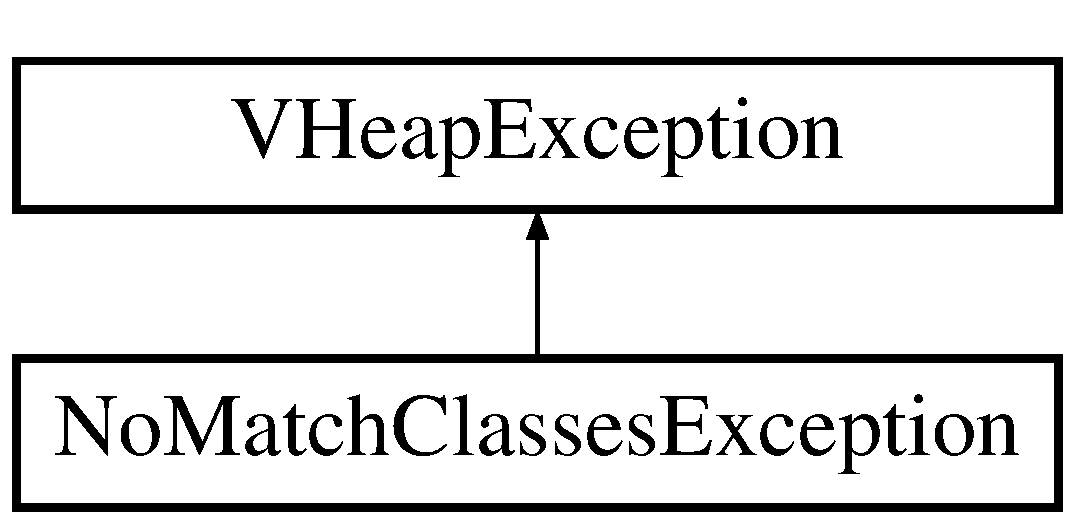
\includegraphics[height=2.000000cm]{class_no_match_classes_exception}
\end{center}
\end{figure}
\subsection*{Public Member Functions}
\begin{DoxyCompactItemize}
\item 
const char $\ast$ \hyperlink{class_no_match_classes_exception_a1dc1f5956c7e6c2a9211432471a60e6d}{what} ()
\begin{DoxyCompactList}\small\item\em Es el metodo que contiene el mensaje de error de la clase. \end{DoxyCompactList}\end{DoxyCompactItemize}


\subsection{Detailed Description}
Es la clase que representa al error cuando dos objeto no pertenecen a la misma clase. 

\subsection{Member Function Documentation}
\hypertarget{class_no_match_classes_exception_a1dc1f5956c7e6c2a9211432471a60e6d}{\index{No\-Match\-Classes\-Exception@{No\-Match\-Classes\-Exception}!what@{what}}
\index{what@{what}!NoMatchClassesException@{No\-Match\-Classes\-Exception}}
\subsubsection[{what}]{\setlength{\rightskip}{0pt plus 5cm}const char$\ast$ No\-Match\-Classes\-Exception\-::what (
\begin{DoxyParamCaption}
{}
\end{DoxyParamCaption}
)\hspace{0.3cm}{\ttfamily [inline]}, {\ttfamily [virtual]}}}\label{class_no_match_classes_exception_a1dc1f5956c7e6c2a9211432471a60e6d}


Es el metodo que contiene el mensaje de error de la clase. 

\begin{DoxyReturn}{Returns}
una cadena de caracteres que contiene el error 
\end{DoxyReturn}


Reimplemented from \hyperlink{class_v_heap_exception_a58154e8dc02f9c28dfefad7897f8b2cf}{V\-Heap\-Exception}.



The documentation for this class was generated from the following file\-:\begin{DoxyCompactItemize}
\item 
src/nomatchclassesexception.\-h\end{DoxyCompactItemize}

\hypertarget{class_null_pointer_exception}{\section{Null\-Pointer\-Exception Class Reference}
\label{class_null_pointer_exception}\index{Null\-Pointer\-Exception@{Null\-Pointer\-Exception}}
}


La clase \hyperlink{class_null_pointer_exception}{Null\-Pointer\-Exception}, representa al error que se envia cuando se accesa a una porcion de memoria a la cual no se puede accesar.  




{\ttfamily \#include $<$nullpointerexception.\-h$>$}

Inheritance diagram for Null\-Pointer\-Exception\-:\begin{figure}[H]
\begin{center}
\leavevmode
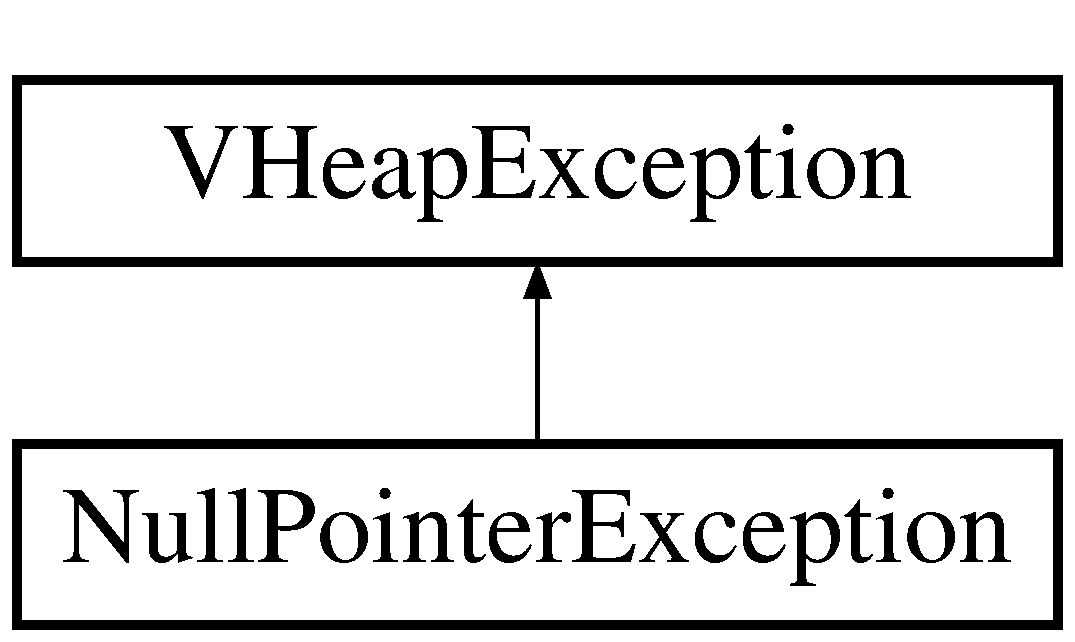
\includegraphics[height=2.000000cm]{class_null_pointer_exception}
\end{center}
\end{figure}
\subsection*{Public Member Functions}
\begin{DoxyCompactItemize}
\item 
const char $\ast$ \hyperlink{class_null_pointer_exception_a0dcc55bb0f3a50e888d8d4a904508313}{what} ()
\begin{DoxyCompactList}\small\item\em Es el metodo que contiene el mensaje de error de la clase. \end{DoxyCompactList}\end{DoxyCompactItemize}


\subsection{Detailed Description}
La clase \hyperlink{class_null_pointer_exception}{Null\-Pointer\-Exception}, representa al error que se envia cuando se accesa a una porcion de memoria a la cual no se puede accesar. 

\subsection{Member Function Documentation}
\hypertarget{class_null_pointer_exception_a0dcc55bb0f3a50e888d8d4a904508313}{\index{Null\-Pointer\-Exception@{Null\-Pointer\-Exception}!what@{what}}
\index{what@{what}!NullPointerException@{Null\-Pointer\-Exception}}
\subsubsection[{what}]{\setlength{\rightskip}{0pt plus 5cm}const char$\ast$ Null\-Pointer\-Exception\-::what (
\begin{DoxyParamCaption}
{}
\end{DoxyParamCaption}
)\hspace{0.3cm}{\ttfamily [inline]}, {\ttfamily [virtual]}}}\label{class_null_pointer_exception_a0dcc55bb0f3a50e888d8d4a904508313}


Es el metodo que contiene el mensaje de error de la clase. 

\begin{DoxyReturn}{Returns}
una cadena de caracteres que contiene el error 
\end{DoxyReturn}


Reimplemented from \hyperlink{class_v_heap_exception_a58154e8dc02f9c28dfefad7897f8b2cf}{V\-Heap\-Exception}.



The documentation for this class was generated from the following file\-:\begin{DoxyCompactItemize}
\item 
src/nullpointerexception.\-h\end{DoxyCompactItemize}

\hypertarget{classv_char}{\section{v\-Char Class Reference}
\label{classv_char}\index{v\-Char@{v\-Char}}
}


The documentation for this class was generated from the following files\-:\begin{DoxyCompactItemize}
\item 
src/vchar.\-h\item 
src/vchar.\-cpp\end{DoxyCompactItemize}

\hypertarget{classv_heap}{\section{v\-Heap Class Reference}
\label{classv_heap}\index{v\-Heap@{v\-Heap}}
}


La clase \hyperlink{classv_heap}{v\-Heap}, Representa a un manejador de memoria. Cuenta con un compresor de memoria, garbage collector y los metodos escenciales.  




{\ttfamily \#include $<$vheap.\-h$>$}

\subsection*{Public Member Functions}
\begin{DoxyCompactItemize}
\item 
\hyperlink{classv_ref}{v\-Ref} \hyperlink{classv_heap_ae4aae8ea89bc24fffed43c509fdfdc8c}{v\-Malloc} (unsigned int p\-Size, string p\-Type)
\begin{DoxyCompactList}\small\item\em Reserva memoria en el \hyperlink{classv_heap}{v\-Heap}, ademas crea un objeto que pertenece a la clase \hyperlink{class_minimalism_bit_vector}{que representa al objeto en memoria, contando con un id, contador de referencias, offset en memoria etc. }\end{DoxyCompactList}\item 
void \hyperlink{classv_heap_abb964cfa76ddee4cd1cc22dae845eed4}{v\-Free} (\hyperlink{classv_ref}{v\-Ref} $\ast$p\-Ref)
\begin{DoxyCompactList}\small\item\em Libera la memoria que un \hyperlink{classv_ref}{v\-Ref} apunta, si la referencia no existe no hace nada. \end{DoxyCompactList}\item 
void \hyperlink{classv_heap_aba09b3334fc1a732308f278c9e292484}{set} (\hyperlink{classv_ref}{v\-Ref} $\ast$p\-Ref, const \hyperlink{classv_object}{v\-Object} $\ast$p\-Object)
\begin{DoxyCompactList}\small\item\em setea el contenido de un \hyperlink{classv_ref}{v\-Ref} \end{DoxyCompactList}\item 
\hyperlink{classv_object}{v\-Object} $\ast$ \hyperlink{classv_heap_ad37c93fe08d1b15f4785a58e865f14f1}{get} (\hyperlink{classv_ref}{v\-Ref} $\ast$p\-Ref)
\begin{DoxyCompactList}\small\item\em Obtiene el objeto contenido en el \hyperlink{classv_ref}{v\-Ref}, si el \hyperlink{classv_ref}{v\-Ref} es invalido, o sea que ya se ha borrado o es una referencia nula se lanza un error de \hyperlink{class_null_pointer_exception}{Null\-Pointer\-Exception}. \end{DoxyCompactList}\item 
void \hyperlink{classv_heap_a4691f4ba088fe19eb2bcaedf90205eb5}{add\-Ref} (const \hyperlink{classv_ref}{v\-Ref} $\ast$p\-Ref)
\begin{DoxyCompactList}\small\item\em agrega una referencia a la referencia pasada por el parametro, si la referencia pasada por el parametro es nula entonces no se hace nada \end{DoxyCompactList}\item 
bool \hyperlink{classv_heap_a56ee2409f56a8117fd3b04434803b3ba}{protect} (\hyperlink{classv_ref}{v\-Ref} $\ast$p\-V\-Ref)
\begin{DoxyCompactList}\small\item\em protect Protege una zona de memoria. \end{DoxyCompactList}\item 
void \hyperlink{classv_heap_a156d31e57a36f093898e4b302e5f270a}{remove\-Reference} (\hyperlink{classv_ref}{v\-Ref} $\ast$p\-V\-Ref)
\begin{DoxyCompactList}\small\item\em remove\-Reference Elimina la refencia hace que el conteo de referencias hacia lo que apunta el \hyperlink{classv_ref}{v\-Ref} sea disminuido en 1 \end{DoxyCompactList}\item 
\hypertarget{classv_heap_af893c48a50166f6e144829e070afa0f0}{void \hyperlink{classv_heap_af893c48a50166f6e144829e070afa0f0}{collect\-Garbage} ()}\label{classv_heap_af893c48a50166f6e144829e070afa0f0}

\begin{DoxyCompactList}\small\item\em es el metodo que lleva a cabo la accion que se le asigna al \hyperlink{class_garbage_collector_thread}{Garbage\-Collector\-Thread}\end{DoxyCompactList}\item 
\hypertarget{classv_heap_ac64f5a67b13397c87cfe594dab278020}{void \hyperlink{classv_heap_ac64f5a67b13397c87cfe594dab278020}{compact} ()}\label{classv_heap_ac64f5a67b13397c87cfe594dab278020}

\begin{DoxyCompactList}\small\item\em Es el metodo que se encarga de realizar las tareas asignadas al compactador de memoria \hyperlink{}{memory\-Compactor.}\end{DoxyCompactList}\item 
bool \hyperlink{classv_heap_a4e451a077578bc4e286de41a0b3ebe33}{is\-Running} ()
\begin{DoxyCompactList}\small\item\em verifica si el \hyperlink{classv_heap}{v\-Heap} sigue corriendo \end{DoxyCompactList}\item 
\hypertarget{classv_heap_aea047ac5e0f6cc9c8ac39a8984c8cedc}{void \hyperlink{classv_heap_aea047ac5e0f6cc9c8ac39a8984c8cedc}{print} ()}\label{classv_heap_aea047ac5e0f6cc9c8ac39a8984c8cedc}

\begin{DoxyCompactList}\small\item\em Imprime lo que se encuetra en el \hyperlink{classv_heap}{v\-Heap}. \end{DoxyCompactList}\item 
std\-::string \hyperlink{classv_heap_af6967e0e004d4ae78c88363878ae96a3}{get\-Type} (\hyperlink{classv_ref}{v\-Ref} $\ast$p\-Ref)
\begin{DoxyCompactList}\small\item\em Obtiene un string con el tipo de dato de la referencia. \end{DoxyCompactList}\item 
unsigned int \hyperlink{classv_heap_ae9f9f3ed79f45beb7b47e88a590fac61}{get\-Wight} (\hyperlink{classv_ref}{v\-Ref} $\ast$p\-Ref)
\begin{DoxyCompactList}\small\item\em Obtiene un unsigned int que representa el peso de la referencia. \end{DoxyCompactList}\item 
\hypertarget{classv_heap_a8bbcf6e79d6d28f16a1de164619e04ef}{virtual \hyperlink{classv_heap_a8bbcf6e79d6d28f16a1de164619e04ef}{$\sim$v\-Heap} ()}\label{classv_heap_a8bbcf6e79d6d28f16a1de164619e04ef}

\begin{DoxyCompactList}\small\item\em $\sim$v\-Heap, detiene los threads, setea en false la bandera del \hyperlink{classv_heap}{v\-Heap} la cual dice si el \hyperlink{classv_heap}{v\-Heap} esta corriendo, Libera la memoria que ocupa. Bloquea todo el proceso con mutex \end{DoxyCompactList}\end{DoxyCompactItemize}
\subsection*{Static Public Member Functions}
\begin{DoxyCompactItemize}
\item 
static \hyperlink{classv_heap}{v\-Heap} $\ast$ \hyperlink{classv_heap_a1b50fb6f333ab744a080647f689f3de9}{get\-Instance} ()
\begin{DoxyCompactList}\small\item\em Obtiene la unica instancia, si no exite la crea. \end{DoxyCompactList}\end{DoxyCompactItemize}
\subsection*{Static Public Attributes}
\begin{DoxyCompactItemize}
\item 
\hypertarget{classv_heap_a2ab6fdef3b9adac6392f2c7a0bf43c1c}{static pthread\-\_\-mutex\-\_\-t \hyperlink{classv_heap_a2ab6fdef3b9adac6392f2c7a0bf43c1c}{mut} = P\-T\-H\-R\-E\-A\-D\-\_\-\-M\-U\-T\-E\-X\-\_\-\-I\-N\-I\-T\-I\-A\-L\-I\-Z\-E\-R}\label{classv_heap_a2ab6fdef3b9adac6392f2c7a0bf43c1c}

\begin{DoxyCompactList}\small\item\em mut, Es el mutex de la clase, todos los metodos de la clase estan protegidos por el mutex \end{DoxyCompactList}\end{DoxyCompactItemize}


\subsection{Detailed Description}
La clase \hyperlink{classv_heap}{v\-Heap}, Representa a un manejador de memoria. Cuenta con un compresor de memoria, garbage collector y los metodos escenciales. 

\subsection{Member Function Documentation}
\hypertarget{classv_heap_a4691f4ba088fe19eb2bcaedf90205eb5}{\index{v\-Heap@{v\-Heap}!add\-Ref@{add\-Ref}}
\index{add\-Ref@{add\-Ref}!vHeap@{v\-Heap}}
\subsubsection[{add\-Ref}]{\setlength{\rightskip}{0pt plus 5cm}void v\-Heap\-::add\-Ref (
\begin{DoxyParamCaption}
\item[{const {\bf v\-Ref} $\ast$}]{p\-Ref}
\end{DoxyParamCaption}
)}}\label{classv_heap_a4691f4ba088fe19eb2bcaedf90205eb5}


agrega una referencia a la referencia pasada por el parametro, si la referencia pasada por el parametro es nula entonces no se hace nada 


\begin{DoxyParams}{Parameters}
{\em p\-Ref} & el \hyperlink{classv_ref}{v\-Ref} al cual se desea agregar una referencia mas \\
\hline
\end{DoxyParams}
\hypertarget{classv_heap_ad37c93fe08d1b15f4785a58e865f14f1}{\index{v\-Heap@{v\-Heap}!get@{get}}
\index{get@{get}!vHeap@{v\-Heap}}
\subsubsection[{get}]{\setlength{\rightskip}{0pt plus 5cm}{\bf v\-Object} $\ast$ v\-Heap\-::get (
\begin{DoxyParamCaption}
\item[{{\bf v\-Ref} $\ast$}]{p\-Ref}
\end{DoxyParamCaption}
)}}\label{classv_heap_ad37c93fe08d1b15f4785a58e865f14f1}


Obtiene el objeto contenido en el \hyperlink{classv_ref}{v\-Ref}, si el \hyperlink{classv_ref}{v\-Ref} es invalido, o sea que ya se ha borrado o es una referencia nula se lanza un error de \hyperlink{class_null_pointer_exception}{Null\-Pointer\-Exception}. 


\begin{DoxyParams}{Parameters}
{\em p\-Ref} & el puntero de la \hyperlink{classv_ref}{v\-Ref} de la cual se quiere conseguir el \hyperlink{classv_object}{v\-Object} \\
\hline
\end{DoxyParams}

\begin{DoxyExceptions}{Exceptions}
{\em \hyperlink{class_null_pointer_exception}{Null\-Pointer\-Exception}} & si el \hyperlink{classv_ref}{v\-Ref} apunta a algun dato no existente en el \hyperlink{classv_heap}{v\-Heap} \\
\hline
\end{DoxyExceptions}
\begin{DoxyReturn}{Returns}
el Objeto al cual p\-Ref \char`\"{}apunta\char`\"{} 
\end{DoxyReturn}
\hypertarget{classv_heap_a1b50fb6f333ab744a080647f689f3de9}{\index{v\-Heap@{v\-Heap}!get\-Instance@{get\-Instance}}
\index{get\-Instance@{get\-Instance}!vHeap@{v\-Heap}}
\subsubsection[{get\-Instance}]{\setlength{\rightskip}{0pt plus 5cm}{\bf v\-Heap} $\ast$ v\-Heap\-::get\-Instance (
\begin{DoxyParamCaption}
{}
\end{DoxyParamCaption}
)\hspace{0.3cm}{\ttfamily [static]}}}\label{classv_heap_a1b50fb6f333ab744a080647f689f3de9}


Obtiene la unica instancia, si no exite la crea. 

\begin{DoxyReturn}{Returns}
el puntero a la unica instancia 
\end{DoxyReturn}
\hypertarget{classv_heap_af6967e0e004d4ae78c88363878ae96a3}{\index{v\-Heap@{v\-Heap}!get\-Type@{get\-Type}}
\index{get\-Type@{get\-Type}!vHeap@{v\-Heap}}
\subsubsection[{get\-Type}]{\setlength{\rightskip}{0pt plus 5cm}std\-::string v\-Heap\-::get\-Type (
\begin{DoxyParamCaption}
\item[{{\bf v\-Ref} $\ast$}]{p\-Ref}
\end{DoxyParamCaption}
)}}\label{classv_heap_af6967e0e004d4ae78c88363878ae96a3}


Obtiene un string con el tipo de dato de la referencia. 


\begin{DoxyParams}{Parameters}
{\em p\-Ref} & es la referencia de la cual se quiere solicitar el tipo de dato \\
\hline
\end{DoxyParams}
\begin{DoxyReturn}{Returns}
el tipo de dato que la referencia apunta 
\end{DoxyReturn}
\hypertarget{classv_heap_ae9f9f3ed79f45beb7b47e88a590fac61}{\index{v\-Heap@{v\-Heap}!get\-Wight@{get\-Wight}}
\index{get\-Wight@{get\-Wight}!vHeap@{v\-Heap}}
\subsubsection[{get\-Wight}]{\setlength{\rightskip}{0pt plus 5cm}unsigned int v\-Heap\-::get\-Wight (
\begin{DoxyParamCaption}
\item[{{\bf v\-Ref} $\ast$}]{p\-Ref}
\end{DoxyParamCaption}
)}}\label{classv_heap_ae9f9f3ed79f45beb7b47e88a590fac61}


Obtiene un unsigned int que representa el peso de la referencia. 


\begin{DoxyParams}{Parameters}
{\em p\-Ref} & es la referencia de la cual se quiere solicitar el peso del objeto \\
\hline
\end{DoxyParams}
\begin{DoxyReturn}{Returns}
el peso del objeto que la referencia apunta 
\end{DoxyReturn}
\hypertarget{classv_heap_a4e451a077578bc4e286de41a0b3ebe33}{\index{v\-Heap@{v\-Heap}!is\-Running@{is\-Running}}
\index{is\-Running@{is\-Running}!vHeap@{v\-Heap}}
\subsubsection[{is\-Running}]{\setlength{\rightskip}{0pt plus 5cm}bool v\-Heap\-::is\-Running (
\begin{DoxyParamCaption}
{}
\end{DoxyParamCaption}
)\hspace{0.3cm}{\ttfamily [inline]}}}\label{classv_heap_a4e451a077578bc4e286de41a0b3ebe33}


verifica si el \hyperlink{classv_heap}{v\-Heap} sigue corriendo 

\begin{DoxyReturn}{Returns}
true, si el \hyperlink{classv_heap}{v\-Heap} se mantiene activo 
\end{DoxyReturn}
\hypertarget{classv_heap_a56ee2409f56a8117fd3b04434803b3ba}{\index{v\-Heap@{v\-Heap}!protect@{protect}}
\index{protect@{protect}!vHeap@{v\-Heap}}
\subsubsection[{protect}]{\setlength{\rightskip}{0pt plus 5cm}bool v\-Heap\-::protect (
\begin{DoxyParamCaption}
\item[{{\bf v\-Ref} $\ast$}]{p\-V\-Ref}
\end{DoxyParamCaption}
)}}\label{classv_heap_a56ee2409f56a8117fd3b04434803b3ba}


protect Protege una zona de memoria. 


\begin{DoxyParams}{Parameters}
{\em p\-V\-Ref} & la referencia que pide la proteccion de la variable \\
\hline
\end{DoxyParams}
\begin{DoxyReturn}{Returns}
true si la zona de memoria se pudo proteger, false si la zona de memoria ya estaba protegida 
\end{DoxyReturn}
\hypertarget{classv_heap_a156d31e57a36f093898e4b302e5f270a}{\index{v\-Heap@{v\-Heap}!remove\-Reference@{remove\-Reference}}
\index{remove\-Reference@{remove\-Reference}!vHeap@{v\-Heap}}
\subsubsection[{remove\-Reference}]{\setlength{\rightskip}{0pt plus 5cm}void v\-Heap\-::remove\-Reference (
\begin{DoxyParamCaption}
\item[{{\bf v\-Ref} $\ast$}]{p\-V\-Ref}
\end{DoxyParamCaption}
)}}\label{classv_heap_a156d31e57a36f093898e4b302e5f270a}


remove\-Reference Elimina la refencia hace que el conteo de referencias hacia lo que apunta el \hyperlink{classv_ref}{v\-Ref} sea disminuido en 1 


\begin{DoxyParams}{Parameters}
{\em p\-V\-Ref} & la referencia que quiere disminuir la referencia \\
\hline
\end{DoxyParams}
\hypertarget{classv_heap_aba09b3334fc1a732308f278c9e292484}{\index{v\-Heap@{v\-Heap}!set@{set}}
\index{set@{set}!vHeap@{v\-Heap}}
\subsubsection[{set}]{\setlength{\rightskip}{0pt plus 5cm}void v\-Heap\-::set (
\begin{DoxyParamCaption}
\item[{{\bf v\-Ref} $\ast$}]{p\-Ref, }
\item[{const {\bf v\-Object} $\ast$}]{p\-Object}
\end{DoxyParamCaption}
)}}\label{classv_heap_aba09b3334fc1a732308f278c9e292484}


setea el contenido de un \hyperlink{classv_ref}{v\-Ref} 


\begin{DoxyParams}{Parameters}
{\em p\-Ref} & la referencia a la cual se quiere setear un dato \\
\hline
{\em p\-Object} & es el objeto que se sobrescribira en la zona de memoria que representa el \hyperlink{classv_ref}{v\-Ref} \\
\hline
\end{DoxyParams}

\begin{DoxyExceptions}{Exceptions}
{\em \hyperlink{class_null_pointer_exception}{Null\-Pointer\-Exception}} & si la referencia es nula o si esta no existe \\
\hline
{\em \hyperlink{class_no_match_classes_exception}{No\-Match\-Classes\-Exception}} & si la clase que el vref representa es diferente de la clase a la cual el \hyperlink{classv_object}{v\-Object} pertenece \\
\hline
\end{DoxyExceptions}
\hypertarget{classv_heap_abb964cfa76ddee4cd1cc22dae845eed4}{\index{v\-Heap@{v\-Heap}!v\-Free@{v\-Free}}
\index{v\-Free@{v\-Free}!vHeap@{v\-Heap}}
\subsubsection[{v\-Free}]{\setlength{\rightskip}{0pt plus 5cm}void v\-Heap\-::v\-Free (
\begin{DoxyParamCaption}
\item[{{\bf v\-Ref} $\ast$}]{p\-Ref}
\end{DoxyParamCaption}
)}}\label{classv_heap_abb964cfa76ddee4cd1cc22dae845eed4}


Libera la memoria que un \hyperlink{classv_ref}{v\-Ref} apunta, si la referencia no existe no hace nada. 


\begin{DoxyParams}{Parameters}
{\em p\-Ref} & es el puntero de un \hyperlink{classv_ref}{v\-Ref} a liberar de la memoria que contiene el \hyperlink{classv_heap}{v\-Heap} \\
\hline
\end{DoxyParams}
\begin{DoxySeeAlso}{See Also}
\hyperlink{classv_ref}{v\-Ref} 
\end{DoxySeeAlso}
\hypertarget{classv_heap_ae4aae8ea89bc24fffed43c509fdfdc8c}{\index{v\-Heap@{v\-Heap}!v\-Malloc@{v\-Malloc}}
\index{v\-Malloc@{v\-Malloc}!vHeap@{v\-Heap}}
\subsubsection[{v\-Malloc}]{\setlength{\rightskip}{0pt plus 5cm}{\bf v\-Ref} v\-Heap\-::v\-Malloc (
\begin{DoxyParamCaption}
\item[{unsigned int}]{p\-Size, }
\item[{string}]{p\-Type}
\end{DoxyParamCaption}
)}}\label{classv_heap_ae4aae8ea89bc24fffed43c509fdfdc8c}


Reserva memoria en el \hyperlink{classv_heap}{v\-Heap}, ademas crea un objeto que pertenece a la clase \hyperlink{class_minimalism_bit_vector}{que representa al objeto en memoria, contando con un id, contador de referencias, offset en memoria etc. }


\begin{DoxyParams}{Parameters}
{\em p\-Size} & es el tamanio de memoria a reservar \\
\hline
{\em p\-Type} & es el tipo de objeto a reservar \\
\hline
\end{DoxyParams}
\begin{DoxyReturn}{Returns}
un \hyperlink{classv_ref}{v\-Ref} que representa un puntero a la memoria reservada por este puntero 
\end{DoxyReturn}
if (!iterator-\/$>$has\-Next() \&\& (iterator-\/$>$get\-Current().Offset() -\/ (tmp1.\-Offset()+tmp1.get\-Weight()) $<$= p\-Size))\{ tmp1 = iterator-\/$>$get\-Current(); \}

The documentation for this class was generated from the following files\-:\begin{DoxyCompactItemize}
\item 
src/vheap.\-h\item 
src/vheap.\-cpp\end{DoxyCompactItemize}

\hypertarget{class_v_heap_exception}{\section{V\-Heap\-Exception Class Reference}
\label{class_v_heap_exception}\index{V\-Heap\-Exception@{V\-Heap\-Exception}}
}


La clase \hyperlink{class_v_heap_exception}{V\-Heap\-Exception}, Representa cualquier error generado por el \hyperlink{classv_heap}{v\-Heap}.  




{\ttfamily \#include $<$vheapexception.\-h$>$}

Inheritance diagram for V\-Heap\-Exception\-:\begin{figure}[H]
\begin{center}
\leavevmode
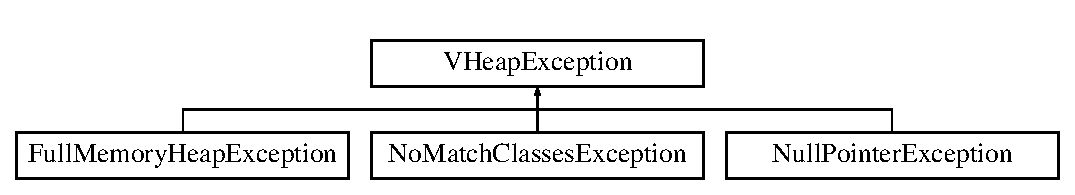
\includegraphics[height=1.085271cm]{class_v_heap_exception}
\end{center}
\end{figure}
\subsection*{Public Member Functions}
\begin{DoxyCompactItemize}
\item 
virtual const char $\ast$ \hyperlink{class_v_heap_exception_a58154e8dc02f9c28dfefad7897f8b2cf}{what} ()
\begin{DoxyCompactList}\small\item\em Es el metodo que contiene el mensaje de error de la clase. \end{DoxyCompactList}\end{DoxyCompactItemize}


\subsection{Detailed Description}
La clase \hyperlink{class_v_heap_exception}{V\-Heap\-Exception}, Representa cualquier error generado por el \hyperlink{classv_heap}{v\-Heap}. 

\subsection{Member Function Documentation}
\hypertarget{class_v_heap_exception_a58154e8dc02f9c28dfefad7897f8b2cf}{\index{V\-Heap\-Exception@{V\-Heap\-Exception}!what@{what}}
\index{what@{what}!VHeapException@{V\-Heap\-Exception}}
\subsubsection[{what}]{\setlength{\rightskip}{0pt plus 5cm}virtual const char$\ast$ V\-Heap\-Exception\-::what (
\begin{DoxyParamCaption}
{}
\end{DoxyParamCaption}
)\hspace{0.3cm}{\ttfamily [inline]}, {\ttfamily [virtual]}}}\label{class_v_heap_exception_a58154e8dc02f9c28dfefad7897f8b2cf}


Es el metodo que contiene el mensaje de error de la clase. 

\begin{DoxyReturn}{Returns}
una cadena de caracteres que contiene el error 
\end{DoxyReturn}


Reimplemented in \hyperlink{class_no_match_classes_exception_a1dc1f5956c7e6c2a9211432471a60e6d}{No\-Match\-Classes\-Exception}, \hyperlink{class_null_pointer_exception_a0dcc55bb0f3a50e888d8d4a904508313}{Null\-Pointer\-Exception}, \hyperlink{class_full_memory_heap_exception_a66ee760289cae528c31ffdedfc2ccc0a}{Full\-Memory\-Heap\-Exception}, \hyperlink{class_index_out_bounds_a0d2a6f3a345d776daf642e6210aad2f2}{Index\-Out\-Bounds}, \hyperlink{class_array_declaration_is_invalid_a74bc87f5d88b08be96bf2178b23f20e9}{Array\-Declaration\-Is\-Invalid}, and \hyperlink{class_array_size_no_compatible_a615b33706018426059fe78a13edf4549}{Array\-Size\-No\-Compatible}.



The documentation for this class was generated from the following file\-:\begin{DoxyCompactItemize}
\item 
src/vheapexception.\-h\end{DoxyCompactItemize}

\hypertarget{classv_int}{\section{v\-Int Class Reference}
\label{classv_int}\index{v\-Int@{v\-Int}}
}


es la clase que representa al int comun  




{\ttfamily \#include $<$vint.\-h$>$}

Inheritance diagram for v\-Int\-:\begin{figure}[H]
\begin{center}
\leavevmode
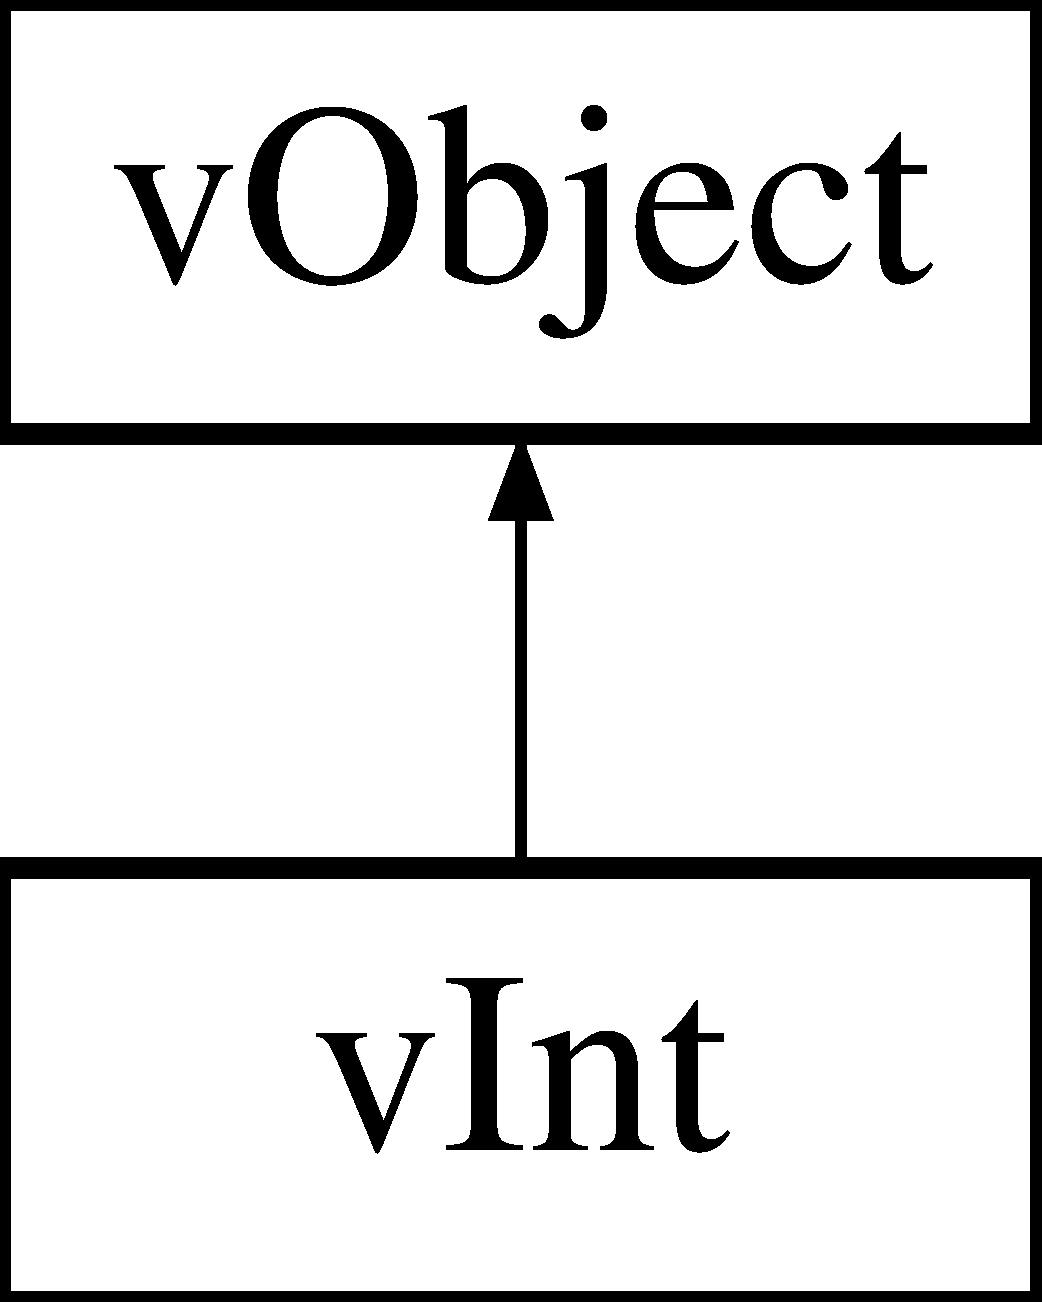
\includegraphics[height=2.000000cm]{classv_int}
\end{center}
\end{figure}
\subsection*{Public Member Functions}
\begin{DoxyCompactItemize}
\item 
\hyperlink{classv_int_a6b689f162fca003015d4f9545b6b846a}{v\-Int} (int p\-Int)
\begin{DoxyCompactList}\small\item\em Es el contructor de \hyperlink{classv_int}{v\-Int}. \end{DoxyCompactList}\item 
int \hyperlink{classv_int_a836fcc7e9a1c6c25de0149e0691a44ec}{get\-Int} ()
\begin{DoxyCompactList}\small\item\em obtiene el int contenido \end{DoxyCompactList}\item 
void \hyperlink{classv_int_a9781020db0c2c20724e4055b0cd82667}{set\-Int} (int p\-Int)
\begin{DoxyCompactList}\small\item\em setea el int contenido \end{DoxyCompactList}\end{DoxyCompactItemize}


\subsection{Detailed Description}
es la clase que representa al int comun 

\subsection{Constructor \& Destructor Documentation}
\hypertarget{classv_int_a6b689f162fca003015d4f9545b6b846a}{\index{v\-Int@{v\-Int}!v\-Int@{v\-Int}}
\index{v\-Int@{v\-Int}!vInt@{v\-Int}}
\subsubsection[{v\-Int}]{\setlength{\rightskip}{0pt plus 5cm}v\-Int\-::v\-Int (
\begin{DoxyParamCaption}
\item[{int}]{p\-Int}
\end{DoxyParamCaption}
)}}\label{classv_int_a6b689f162fca003015d4f9545b6b846a}


Es el contructor de \hyperlink{classv_int}{v\-Int}. 


\begin{DoxyParams}{Parameters}
{\em p\-Int} & es el int a contener \\
\hline
\end{DoxyParams}


\subsection{Member Function Documentation}
\hypertarget{classv_int_a836fcc7e9a1c6c25de0149e0691a44ec}{\index{v\-Int@{v\-Int}!get\-Int@{get\-Int}}
\index{get\-Int@{get\-Int}!vInt@{v\-Int}}
\subsubsection[{get\-Int}]{\setlength{\rightskip}{0pt plus 5cm}int v\-Int\-::get\-Int (
\begin{DoxyParamCaption}
{}
\end{DoxyParamCaption}
)\hspace{0.3cm}{\ttfamily [inline]}}}\label{classv_int_a836fcc7e9a1c6c25de0149e0691a44ec}


obtiene el int contenido 

\begin{DoxyReturn}{Returns}
el int contenido 
\end{DoxyReturn}
\hypertarget{classv_int_a9781020db0c2c20724e4055b0cd82667}{\index{v\-Int@{v\-Int}!set\-Int@{set\-Int}}
\index{set\-Int@{set\-Int}!vInt@{v\-Int}}
\subsubsection[{set\-Int}]{\setlength{\rightskip}{0pt plus 5cm}void v\-Int\-::set\-Int (
\begin{DoxyParamCaption}
\item[{int}]{p\-Int}
\end{DoxyParamCaption}
)\hspace{0.3cm}{\ttfamily [inline]}}}\label{classv_int_a9781020db0c2c20724e4055b0cd82667}


setea el int contenido 


\begin{DoxyParams}{Parameters}
{\em p\-Int} & es el dato nuevo que se quiere setear \\
\hline
\end{DoxyParams}


The documentation for this class was generated from the following files\-:\begin{DoxyCompactItemize}
\item 
src/vint.\-h\item 
src/vint.\-cpp\end{DoxyCompactItemize}

\hypertarget{classv_object}{\section{v\-Object Class Reference}
\label{classv_object}\index{v\-Object@{v\-Object}}
}


Es la clase que representa al objeto contenido en el \hyperlink{classv_heap}{v\-Heap}.  




{\ttfamily \#include $<$vobject.\-h$>$}

Inheritance diagram for v\-Object\-:\begin{figure}[H]
\begin{center}
\leavevmode
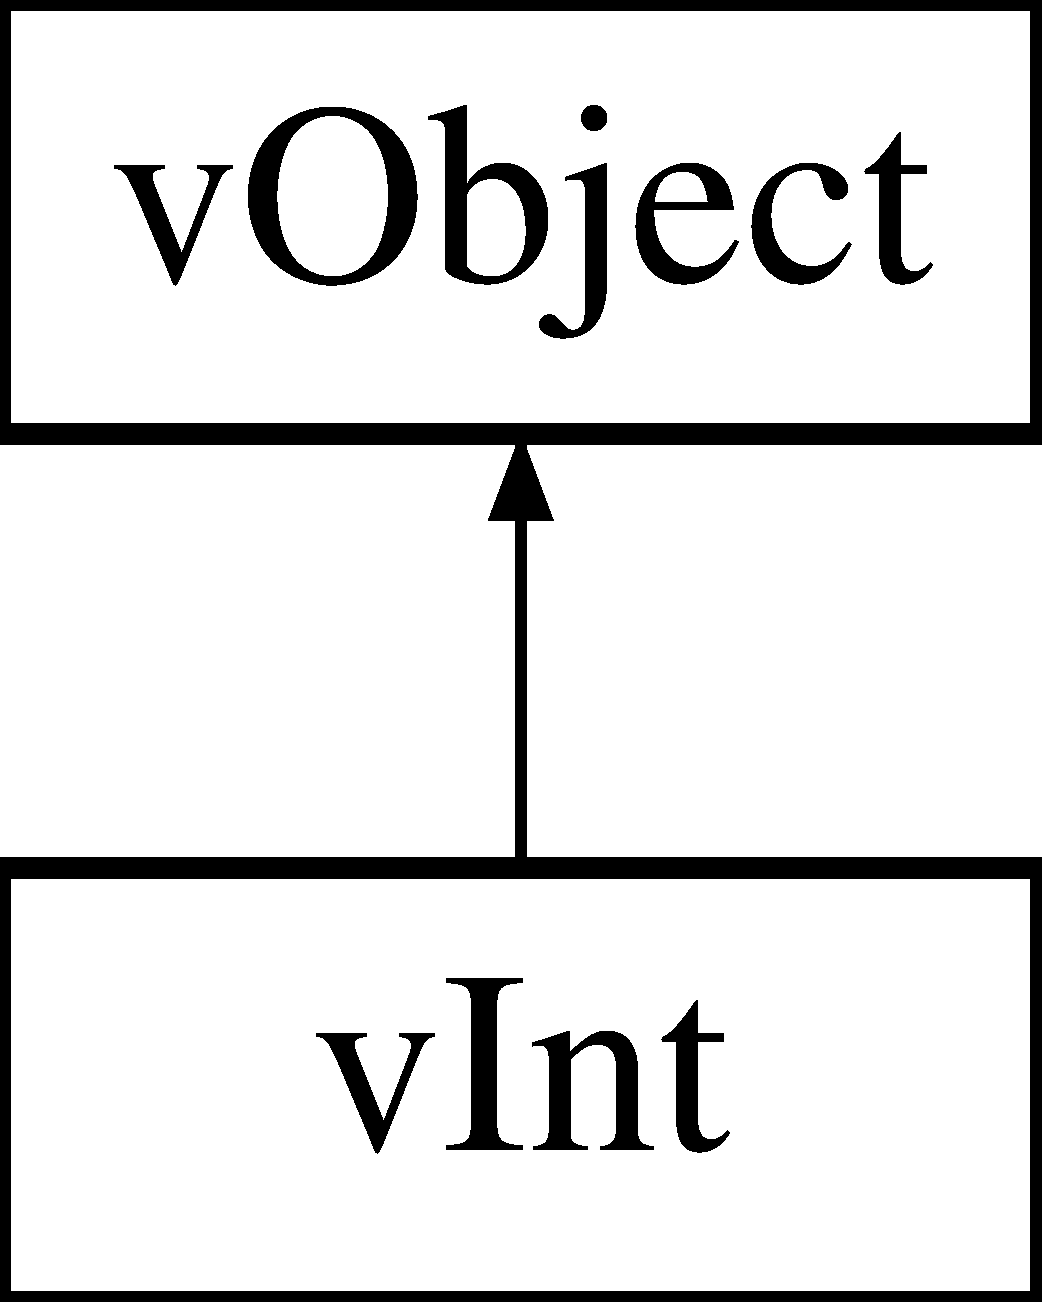
\includegraphics[height=2.000000cm]{classv_object}
\end{center}
\end{figure}
\subsection*{Public Member Functions}
\begin{DoxyCompactItemize}
\item 
\hypertarget{classv_object_af5d1cd42c54c5e33da3dfe5ce747acad}{\hyperlink{classv_object_af5d1cd42c54c5e33da3dfe5ce747acad}{v\-Object} ()}\label{classv_object_af5d1cd42c54c5e33da3dfe5ce747acad}

\begin{DoxyCompactList}\small\item\em es el constructor por defecto \end{DoxyCompactList}\item 
virtual const char $\ast$ \hyperlink{classv_object_a839d2dd4f326f6ae698d832744bf59ce}{get\-Type} () const 
\begin{DoxyCompactList}\small\item\em Retorna una cadena con el tipo de dato. \end{DoxyCompactList}\end{DoxyCompactItemize}


\subsection{Detailed Description}
Es la clase que representa al objeto contenido en el \hyperlink{classv_heap}{v\-Heap}. 

\begin{DoxySeeAlso}{See Also}
\hyperlink{classv_heap}{v\-Heap} 
\end{DoxySeeAlso}


\subsection{Member Function Documentation}
\hypertarget{classv_object_a839d2dd4f326f6ae698d832744bf59ce}{\index{v\-Object@{v\-Object}!get\-Type@{get\-Type}}
\index{get\-Type@{get\-Type}!vObject@{v\-Object}}
\subsubsection[{get\-Type}]{\setlength{\rightskip}{0pt plus 5cm}const char $\ast$ v\-Object\-::get\-Type (
\begin{DoxyParamCaption}
{}
\end{DoxyParamCaption}
) const\hspace{0.3cm}{\ttfamily [virtual]}}}\label{classv_object_a839d2dd4f326f6ae698d832744bf59ce}


Retorna una cadena con el tipo de dato. 

\begin{DoxyReturn}{Returns}
el tipo de dato 
\end{DoxyReturn}


The documentation for this class was generated from the following files\-:\begin{DoxyCompactItemize}
\item 
src/vobject.\-h\item 
src/vobject.\-cpp\end{DoxyCompactItemize}

\hypertarget{classv_ref}{\section{v\-Ref Class Reference}
\label{classv_ref}\index{v\-Ref@{v\-Ref}}
}
\subsection*{Public Member Functions}
\begin{DoxyCompactItemize}
\item 
\hypertarget{classv_ref_a42661b55fdd6d60c1b7d34fec5dc6ebb}{{\bfseries v\-Ref} (const void $\ast$p\-Memory\-Section)}\label{classv_ref_a42661b55fdd6d60c1b7d34fec5dc6ebb}

\item 
\hyperlink{classv_ref_a665fe2849fbbabcb1930128b78c144ff}{v\-Ref} (const \hyperlink{classv_ref}{v\-Ref} \&p\-Ref)
\item 
\hypertarget{classv_ref_a6824b37064baf1055c0634d25af33302}{{\bfseries v\-Ref} (const \hyperlink{classv_ref}{v\-Ref} $\ast$p\-Ref)}\label{classv_ref_a6824b37064baf1055c0634d25af33302}

\item 
\hypertarget{classv_ref_a6fdd2c2154bfe2a436684b0a4d8dc44c}{\hyperlink{classv_ref}{v\-Ref} \& {\bfseries operator=} (const \hyperlink{classv_object}{v\-Object} $\ast$p\-V\-Object)}\label{classv_ref_a6fdd2c2154bfe2a436684b0a4d8dc44c}

\item 
\hypertarget{classv_ref_a09a2b66a31121f2ea39db1d2275df018}{\hyperlink{classv_ref}{v\-Ref} \& {\bfseries operator=} (int p\-Address)}\label{classv_ref_a09a2b66a31121f2ea39db1d2275df018}

\item 
\hypertarget{classv_ref_a7a5795eb3d07af12a724006868ed28ba}{\hyperlink{classv_ref}{v\-Ref} \& {\bfseries operator=} (\hyperlink{classv_ref}{v\-Ref} p\-Ref)}\label{classv_ref_a7a5795eb3d07af12a724006868ed28ba}

\item 
\hyperlink{classv_object}{v\-Object} $\ast$ \hyperlink{classv_ref_a8c6c503ee26c2e26bbf336166992f79c}{operator$\ast$} ()
\item 
\hypertarget{classv_ref_a67f7a5cc022f60bfe5a6d1069d97a455}{bool {\bfseries operator==} (const \hyperlink{classv_ref}{v\-Ref} \&p\-V\-Ref)}\label{classv_ref_a67f7a5cc022f60bfe5a6d1069d97a455}

\item 
\hypertarget{classv_ref_a82bfa187c785c2044dde59aa8d993c6a}{unsigned int {\bfseries get\-Weight} ()}\label{classv_ref_a82bfa187c785c2044dde59aa8d993c6a}

\item 
\hypertarget{classv_ref_a29f102a40b30f7662de769fd07f42f0c}{std\-::string {\bfseries get\-Type} ()}\label{classv_ref_a29f102a40b30f7662de769fd07f42f0c}

\end{DoxyCompactItemize}
\subsection*{Static Public Member Functions}
\begin{DoxyCompactItemize}
\item 
\hypertarget{classv_ref_aa3ac4bab0c6cea635768dbfe40dc1284}{static \hyperlink{classv_ref}{v\-Ref} {\bfseries assing} (size\-\_\-t p\-Size, const \hyperlink{classv_object}{v\-Object} $\ast$p\-V\-Object)}\label{classv_ref_aa3ac4bab0c6cea635768dbfe40dc1284}

\end{DoxyCompactItemize}
\subsection*{Public Attributes}
\begin{DoxyCompactItemize}
\item 
\hypertarget{classv_ref_aaf5d33821d373d8b68daa73b00969c2c}{bool {\bfseries \-\_\-from\-V\-Heap}}\label{classv_ref_aaf5d33821d373d8b68daa73b00969c2c}

\item 
\hypertarget{classv_ref_a3f8a845f0e4623d38404e67ff51d8c5c}{bool {\bfseries \-\_\-destroy\-Ref}}\label{classv_ref_a3f8a845f0e4623d38404e67ff51d8c5c}

\end{DoxyCompactItemize}
\subsection*{Friends}
\begin{DoxyCompactItemize}
\item 
\hypertarget{classv_ref_ad615cc5888405061e930d41dba53d277}{class {\bfseries v\-Heap}}\label{classv_ref_ad615cc5888405061e930d41dba53d277}

\end{DoxyCompactItemize}


\subsection{Constructor \& Destructor Documentation}
\hypertarget{classv_ref_a665fe2849fbbabcb1930128b78c144ff}{\index{v\-Ref@{v\-Ref}!v\-Ref@{v\-Ref}}
\index{v\-Ref@{v\-Ref}!vRef@{v\-Ref}}
\subsubsection[{v\-Ref}]{\setlength{\rightskip}{0pt plus 5cm}v\-Ref\-::v\-Ref (
\begin{DoxyParamCaption}
\item[{const {\bf v\-Ref} \&}]{p\-Ref}
\end{DoxyParamCaption}
)}}\label{classv_ref_a665fe2849fbbabcb1930128b78c144ff}
std\-::cout $<$$<$ \char`\"{}copy is called\char`\"{} $<$$<$ std\-::endl; std\-::cout $<$$<$ \char`\"{}copy amp\char`\"{} $<$$<$ std\-::endl; if (p\-Ref.\-\_\-destroy\-Ref)\hyperlink{classv_heap_a1b50fb6f333ab744a080647f689f3de9}{v\-Heap\-::get\-Instance()}-\/$>$add\-Ref(\&p\-Ref); if(this-\/$>$\-\_\-\-Id == p\-Ref.\-\_\-\-Id)this-\/$>$\-\_\-destroy\-Ref = p\-Ref.\-\_\-destroy\-Ref; else\{ \hyperlink{classv_ref}{v\-Ref} a(this-\/$>$\-\_\-\-Id,false); if (a.\-\_\-\-Id != -\/1)\{ \} std\-::cout $<$$<$ \char`\"{}alguien entra aqui\char`\"{} $<$$<$ std\-::endl; \}

\subsection{Member Function Documentation}
\hypertarget{classv_ref_a8c6c503ee26c2e26bbf336166992f79c}{\index{v\-Ref@{v\-Ref}!operator$\ast$@{operator$\ast$}}
\index{operator$\ast$@{operator$\ast$}!vRef@{v\-Ref}}
\subsubsection[{operator$\ast$}]{\setlength{\rightskip}{0pt plus 5cm}{\bf v\-Object} $\ast$ v\-Ref\-::operator$\ast$ (
\begin{DoxyParamCaption}
{}
\end{DoxyParamCaption}
)}}\label{classv_ref_a8c6c503ee26c2e26bbf336166992f79c}
\hyperlink{classv_ref}{v\-Ref} \&v\-Ref\-::operator =(int p\-Address) \{ \hyperlink{classv_heap_a1b50fb6f333ab744a080647f689f3de9}{v\-Heap\-::get\-Instance()}-\/$>$remove\-Reference(this); this = \hyperlink{classv_heap_a1b50fb6f333ab744a080647f689f3de9}{v\-Heap\-::get\-Instance()}-\/$>$get(p\-Address); return $\ast$this; \} 

The documentation for this class was generated from the following files\-:\begin{DoxyCompactItemize}
\item 
src/vref.\-h\item 
src/vref.\-cpp\end{DoxyCompactItemize}

%--- End generated contents ---

% Index
\newpage
\phantomsection
\addcontentsline{toc}{chapter}{Index}
\printindex

\end{document}
